%You can delete all the comments after you have finished your document
%this sets up the defaults for the documents, 12pt font and A4 size. The article type sets this up as such as opposed to letter or memo.

%for the finer points LaTeX see https://en.wikibooks.org/wiki/LaTeX or http://tex.stackexchange.com/

\documentclass[12pt,a4paper]{article}
\usepackage{titlesec} %these are how we import packages, one helps set up footers and title layout
\usepackage{fancyhdr}

% !TEX TS-program = pdflatex
% !TEX encoding = UTF-8 Unicode
\usepackage[utf8]{inputenc} % set input encoding (not needed with XeLaTeX)

\usepackage{graphicx} % support the \includegraphics command and options
\graphicspath{{./appendicies/}}

% \usepackage[parfill]{parskip} % Activate to begin paragraphs with an empty line rather than an indent

%%% PACKAGES
\usepackage{booktabs} % for much better looking tables
\usepackage[autostyle=false,style=british]{csquotes}
\usepackage{array} % for better arrays (eg matrices) in maths
\usepackage{paralist} % very flexible & customisable lists (eg. enumerate/itemize, etc.)
\usepackage[parfill]{parskip}
\usepackage{verbatim} % adds environment for commenting out blocks of text & for better verbatim
\usepackage{subfig} % make it possible to include more than one captioned figure/table in a single float
\usepackage[toc,page]{appendix}
\usepackage{apalike}
\usepackage{listings}% code listing package
\usepackage{algorithm2e} % algorithm package
% These packages are all incorporated in the memoir class to one degree or another...

\MakeOuterQuote{"}

\newcommand{\figuremacro}[5]{
    \begin{figure}[#1]
        \centering
        \includegraphics[width=#5\columnwidth]{#2}
        \caption[#3]{\textbf{#3}#4}
        \label{fig:#2}
    \end{figure}
}

%header and footer settings
\pagestyle{fancyplain}
\fancyhf{}
\renewcommand{\headrulewidth}{0.5pt}
\renewcommand{\footrulewidth}{0.5pt}
\setlength{\headheight}{15pt}
\fancyhead[L]{Dylan Tyrie-Dron - 40203045}
\fancyhead[R]{ SOC10101 Honours Project}
\fancyfoot[L]{}
\fancyfoot[C]{\vspace{2em}\thepage}

%set better section layout
\makeatletter
\renewcommand\subsection{\@startsection {subsection}{1}{0mm} % name, level, indent
                               {3pt plus 2pt minus 1pt} % before skip
                               {3pt plus 0pt} % after skip
                               {\normalfont\bfseries}}
\makeatother
\makeatletter
\renewcommand\section{\@startsection {section}{1}{0mm} % name, level, indent
                               {4pt plus 2pt minus 1pt} % before skip
                               {4pt plus 0pt} % after skip
                               {\Large\bfseries}}
\makeatother

%put paragraph headings on their own line
\newcommand{\myparagraph}[1]{\paragraph{#1}\mbox{}\\}

% footnote in footer
\newcommand{\fancyfootnotetext}[2]{%
  \fancypagestyle{dingens}{%
    \fancyfoot[LO,RE]{\parbox{12cm}{\footnotemark[#1]\footnotesize #2}}%
  }%
  \thispagestyle{dingens}%
}


%this starts the document
\begin{document}
\lstset{language=Java}

%you can import other documents into your main one, these layout the Title and Declarations on its own page.
%you might need to change these to \ if your on Microsoft Windows.
\newcommand{\HRule}{\rule{\linewidth}{0.5mm}}

\begin{titlepage}
	\begin{center}

	\HRule \\[0.4cm]
    	{\Large \bfseries Adaptation of a Satellite Navigation System\par}
	\vspace{0.2cm}
	\HRule \\[1.5cm]

	
    	\vspace{3cm}
	\begin{minipage}{0.4\textwidth}
	\begin{center} \large
        \emph{}\\
        	Dylan Tyrie-Dron - 40203045
				
   	 \end{center}
    	\end{minipage}
	
	\vspace{2cm}
    	\begin{minipage}{1\textwidth}
    	\begin{center} \large
        
		Submitted in partial fulfilment of \\
		the requirements of Edinburgh Napier University \\
		for the Degree of \\
        	BEng (Hons) Software Engineering
    	\end{center}
    	\end{minipage}

    	\vfill

    	% Bottom of the page
	\begin{minipage}{1\textwidth}
    	\begin{center} \large
		School of Computing
    	\end{center}
    	\end{minipage}
	
	\vspace{1cm}
    	{\large \today}


	\end{center}
\end{titlepage}
%{\large Submitted in partial fulfilment of the requirements of Edinburgh Napier University for the Degree of }

\section*{Authorship Declaration}
\vspace{0.5cm}
\begin{flushleft}
I, (Dylan Tyrie-Dron), confirm that this dissertation and the work presented in it are my own achievement.\newline

Where I have consulted the published work of others this is always clearly attributed;\newline

Where I have quoted from the work of others the source is always given. With the exception of such quotations this dissertation is entirely my own work;\newline

I have acknowledged all main sources of help; \newline

If my research follows on from previous work or is part of a larger collaborative research project I have made clear exactly what was done by others and what I have contributed myself;\newline

I have read and understand the penalties associated with Academic Misconduct.\newline

I also confirm that I have obtained informed consent from all people I have involved in the work in this dissertation following the School's ethical guidelines.\newline
\end{flushleft}

\begin{flushleft} \large
\emph{Signed:} \\
\end{flushleft}

\vspace{.5cm}

\begin{flushleft} \large
\emph{Date:} \\
\end{flushleft}

\vspace{.5cm}

\begin{flushleft} \large
\emph{Matriculation no: }  \\
\end{flushleft}
\pagebreak

\section*{General Data Protection Regulation Declaration}
\vspace{0.5cm}
\begin{flushleft}
Under the General Data Protection Regulation (GDPR) (EU) 2016/679, the University cannot disclose your grade to an unauthorised person. However, other students benefit from studying dissertations that have their grades attached. \newline

\vspace{0.5cm}

Please sign your name below one of the options below to state your preference.\newline
\vspace{0.5cm}

The University may make this dissertation, with indicative grade, available to others.\newline
\vspace{3cm}


The University may make this dissertation available to others, but the grade may not be disclosed.\newline
\vspace{3cm}


The University may not make this dissertation available to others.\newline
\end{flushleft}



\pagebreak

%LaTeX let you define the abstract separately so it wont get sucked into the main document.
\begin{abstract}
% fill the abstract in here
\end{abstract}
\pagebreak

\tableofcontents % is generated for you
\newpage

\listoftables
%generated in same way as figures
\newpage

\listoffigures
%you may have captions such as equations, listings etc they should all appear as required
%these are done for you as long as you use \begin{figure}[placement settings] .. bla bla ... \end{figure}
\newpage

\section*{Acknowledgements}
Insert acknowledgements here
\subsection*{}
	I would like to thank my cat, dog and family.
\newpage


\section{Introduction}

\subsection{Definitions}

\begin{itemize}
  \item \textbf{Application Programming Interface/s (\enquote{API} or \enquote{APIs})} - a programming library,  created to build part of a software application.
  \item \textbf{OpenStreetMap/OpenStreetMaps} - (tbc)
  \item \textbf{Google Maps} - (tbc)
  \item \textbf{TomTom} - (tbc)
  \item \textbf{TomTom Maps} - (tbc)
  \item \textbf{Optimisation?} - (tbc)
  \item \textbf{Open-source?} - (tbc)
\end{itemize}

stat about sat navs and mobile phones to start...
The aim\footnote{testtest} of this project is to adapt a satellite navigation system to provide the most favourable route from one departure point to a set destination. This will be achieved by testing Dijkstra's pathfinding algorithm and optimising it for a navigation system \cite{Dijkstra1959}. Research will also be carried out using traffic and other data to show how vehicles may reach their destinations more quickly. More realistic results may be achieved, by testing, changing algorithmic variables and then then attempting to improve the algorithm through the use of the test data. The results will be evaluated by comparing the test data to similar test data from experiments developed by others, thus determining which method is the most accurate, cost-effective and efficient way of travelling through a city. The main interface used to convey the outcome of this project is an android application. Research will also be undertaken to find out if applications which contain APIs such as: OpenStreetMaps, Google Maps and TomTom Maps may be used to speed up development of the application.

\subsection{Background}

The percentage of households in Britain that own at least one car or van is ever increasing. In 2017, the percentage was 76\%, meaning that there is an increasing need for fast and efficient ways to travel as the roads get inevitably busier (national survey).

The use of navigation applications on mobile phones provides more efficient and portable ways to navigate roads. Navigation applications nowadays have the power to direct and organise their users onto different routes to spread the traffic load on each road and get the mass majority of people to their destinations as fast as possible. However, a car’s speed can also be affected by many other aspects.

The use of optimisation to develop more accurate results based on somewhat unknown factors that affect a car’s speed and therefore may be used as another method to develop more efficient navigation tools.


\subsection{Aims and Objectives}

The aim of this project is to adapt a satellite navigation system to provide the most favourable route to a particular destination. This will be achieved by identifying factors that effect a car’s speed, routing through the use of Dijkstra’s shortest path algorithm and optimising the results. The development may be sped up through the use of an open-source API.
The initial objectives are: 
\begin{itemize}
  \item 	Set up an initial interface to display an optimal route.
  \item Provide an algorithm for which a route can be determined.
  \item Display the routes on the interface.
  \item 	Provide weighting factors to adapt the algorithm and produce a more realistic result.
  \item Use traffic data to provide more realistic routing.
\end{itemize}	

\subsection{Project Scope and Constraints}

A wide verity of tests will produce results for this project. Each test will use a small range of points to reduce computation time. The scope of this project will depend on the restrictions and limitations of the API chosen. 

expand this...

\subsection{Motivation}
\subsection{Report Structure}


\subsection{Summary}
\newpage
\section{Literature Review}

\subsection{Factors affecting the speed of cars on roads}
The speed of cars on roads can be managed by using traffic lights, speed bumps and many more intentional methods put in place by government. However, weather conditions, road incidents and traffic congestion are some of the main factors which affect road users and the speed of cars. These factors are often unpredictable and therefore cannot be reliably calculated by an algorithm before it is presented with them. This suggests that the algorithm may have to adapt in real time to meet users’ demands.

An extension of these factors is the turning path where junctions and roundabouts cause a car’s speed to be affected (factors affecting transportation). Other factors suggested are road quality and turning path. Road quality is important as cars can be slowed down by a road that needs maintenance with road faults such as potholes provide issues for the speed of cars. The construction of a road surface needs to be carefully planned and road surfaces are different depending on what climate a country generally has (factors affecting transportation). 

Based on data in Beijing, 60\% of the total time is spent on intersections. however, 2.7\% of all the intersections were main intersections (400 intersections) and they took 18\% of the total intersection-time suggesting that a large proportion of the total intersection-time was wasted on main intersections \cite{Liu}. This suggests that that another factor that affects car speed is in fact moving from minor roads to major roads. 

In edz however...

\subsection{Algorithms}

Pathfinding is finding the...

explain Dijkstra...
problems with Dijkstra... link into the time-based algorithms...

Data stored in real-time, taken from cars can be stored in a database to affect the routing algorithm: point (long/lat), time stamps, driving speed and orientation\cite{Zheng2018}. This data may be used to form part of a time-based algorithm.

Algorithms that are often used to find the fastest routes are often based on Dijkstra’s original shortest distance algorithm, however, to adapt that to a time-based algorithm it has to accept factors that will change the distance of each road to then find the roads that take the least time. Comparing the two algorithms below, you can see that there is a subtle difference between the way they calculate the “shortest distances”. In Algorithm 1 … in Algorithm 2 … \cite{Zheng2018}.

Heristic1 (time-based algorithm), Heristic2 (time-based algorithm), Dijkstra (distance-based). \cite{Zheng2018}

%lstinputlisting{}


\subsubsection{Distance based algorithm versus time based algorithm}

Due to the nature of the project, the algorithm must be a time-based algorithm and cannot solely rely on the routes with the shortest distance.

There is a difference between distance-based navigation and time-based navigation: graph (a) shows a distance algoithm with the context of navigating through a road network, (b) shows a time algorithm and how a different route is taken (change this) as illustrated in figure 1, the red line highlights the path of navigation of a car from points 0 to 5 and the black denotes other potential routes; although the distance 
of the red line from points 1 to 3 to 5 shown in (a), it takes less time to go from points 1 to 5 as shown in (b), therefore (b) demonstrates the optimum (time-based) route \cite{Zheng2018}. 

\figuremacro{h}{TimevsDistanceWeightFactors}{Time versus Distance graphs}{- These are two graphs that represent distance and time respectively. Adapted from \cite{Zheng2018} and \cite{SpeedvsTime}}{0.6} 

\subsection{Traffic Data}

Mobile applications for Navigation have the power to track where current users are and use previous users’ historic location data to aid in the navigation through congested areas. This can also be done in real time by finding groups of users in the same location.

An example of using users’ current location data to determine the speed weighting for cars on the same street can be seen in this equation \cite{Zheng2018}: 
\[
    SW = \frac{v_{avg}(section)}{(T_c \times v_{avg}(whole street))}
\]

Where ~$SW$ is the speed weighting, ~$v_{arg}(section)$ is the average speed of cars in a section of the current street, ~$T_c$ is the total number of cars on the current street and\newline ~$v_{avg}(whole street)$ is the average speed of cars in the current street. However, this equation assumes that all the car users on the street are using the same application to collect their data. 

There is a small problem with tracking users within one app: other car users may use other navigation applications on the same road. As illustrated in Fig.\ref{fig:tomtomTracking} below there are three users on the road. However, not all users on the road are using the same application and therefore the tracking of users on that road has become inaccurate.

\figuremacro{h}{tomtomTracking}{Car users on one app versus another}{- A map showing one blue cursor representing users from Google maps \footnotemark[1] and two red cursors on the same street. Adapted from \cite{TomTomMyDrive}}{1.0}

\fancyfootnotetext{\value{footnote}}{https://www.google.com/maps}
Traffic congestion can also be measured by detecting the average speed of any of the vehicles on a street. This average speed will then be compared to a traffic congestion speed threshold. If the vehicles are moving slower than that threshold, then a road is deemed to be congested. Deandrea and Marcelloni’s paper suggests the speed threshold is: 10km/h \cite{DAndrea2017}.

In order to build an algorithm to alleviate traffic congestion, it is necessary to set the usual average speed on a road or set of roads ("route A"), then identify the actual speed of cars at a particular time. Cars would then be diverted onto a different route which is closer to the optimum speed (ie. legal speed). The process would be repeated in order to reduce traffic congestion on route A. \cite{Zheng2018}

change this... to not have methods...
Method 1 suggests that from multiple users’ location data you can determine the severity of traffic congestion, however, a simpler technique of just finding any car’s speed and comparing it to a threshold may be easier and more reliable to set up. Consequently, Method 1 seems to be more accurate than method 2 but due to the ease of use and more consistent promise of data, method 2 seems to be a more appropriate method for this project (put this into intro of Methodology) if traffic data is implemented.

\subsubsection{Traffic States}

A lot of the popular satellite navigation applications are similar in determining different levels of traffic \cite{DAndrea2017}. The usual states of traffic that popular systems implement are flowing, slow, very slowed and blocked. Another state that was added in Deandrea and Marcelloni’s paper was absent, which means there is either no traffic or a total absence of vehicles. This is used for incident detection. The usual traffic systems will check the number of vehicles that have crossed a segment in an amount of time.

In Deandrea and Marcelloni’s paper, the system being described checks if there are sufficient vehicles on each road segment and sets the traffic states based on this algorithm:

\begin{algorithm}[H]
  \SetAlgoLined
    \eIf{insufficient number of vechiles on the road}{
      \eIf{0 vechiles}{
        set state to absent\;
      }{
        set to flowing\;
      }
     }{
     Find the median speed of the cars in the road segment ($ms$)\;
     
     Compare $ms$ to a percentage of the currrent road speed limit that is close to the speed limit ($p_1$)\;

     \eIf{percentage of speed limit reached $p_1$ or higher median speed found}{
        set to flowing\;
     }{
       \eIf{median speed is in a lower range ($p_2$) than $p_1$}{
        state is set to slower\;
       }{
         \eIf{median speed is in a lower range ($p_3$) than $p_2$}{
          state is set to very slow\;
         }{
          state is set to blocked\;
         }
       }
     }


    }
   \caption{Find the flow of traffic on a road}
  \end{algorithm}

  Where~$p_1$ = 50\%, $p_2$ = 40\%, $p_3$ = 30\% and the sufficient number of cars on a road was set to 4 \cite{DAndrea2017}.
 

\section{Technology Review}
\subsection{Introduction}
TomTom maps was one of the stand out technologies for this project as it was one of the most accessible and open-source libraries. It also had the capabilities to achieve a large set of the aims that were described at the start of the project.  

Other technologies that were considered were Google maps, HERE maps, OpenStreetMaps and Bing maps. Google maps was thought to be this project’s maps development software at the start of this project, however, the aims of the project could not be developed through Google maps due to the restricted amount of data that could be retrieved from the library. HERE maps was a potential maps development software, however, the initial map application could not be set up, when following the tutorial. OpenStreetMaps had promise as a potential maps development software. It had all the features that all the other maps and more. A feature that could have been useful to this project to help with the application of routing is the fact that OpenStreetMaps has the locations of traffic lights. However, OpenStreetMaps lacked the functionality of other maps as…
\subsection{Comparison of Technologies}
table...
\begin{table}
  
\end{table}

\subsection{Further detail on TomTom maps}
TomTom was founded in 1991 beginning in the business-to-business section of the technology market. They then went on to develop personal digital assistants (PDAS) in the early 90s, going on to become the market leader in PDA software with navigation applications such as "RoutePlanner" and "Citymaps". In 2002, the TomTom "Navigator" provided the first affordable and easy-to-use navigation system to customers in Europe.

This increased demand for portable navigation devices, which lead to the development of the Portable Navigation Device (PND). This became the fastest selling consumer technology device in history and by 2016 TomTom had sold over 78 million PNDs.

Nowadays, TomTom provide customers with several navigation-based products, including a navigation app for android and wrist devices for sports enthusiasts, reaching over 800 million people a day \cite{TomTomHist}.

\subsubsection{Map tiles}
The TomTom maps API provides the user to view the maps using raster tile images or vector tile images. The difference is subtle when viewing the maps, however in theory, raster tiles should be more detailed as the tile is coloured per pixel whereas vector imaging colours the tile based on the objects inside it (roads, rivers, etc).

The number of tiles shown depends on the level of zoom that the user has defined (by using a pinching gesture on the screen). There are 23 different levels of zoom with 0 showing the whole world in one tile and zoom level 22 showing 2 to the power of 22 tiles. 

\figuremacro{h}{TomTomZoom1}{Zoom level 1}{- This is Zoom Level 1 which is 4 tiles in total.}{1.0} 

\subsubsection{Map layers}
The TomTom maps API also allows the maps to be separated into different layers to make it easier to update the map or to show places in different languages etc. There are three layers defined in the TomTom documentation: Basic, Hybrid and Labels. The Basic layer shows all the maps features as an end user would see it. The Hybrid layer is a step down from that as it takes the polygons that outline the birds eye view of the buildings so that the view of the map is focussed on the roads more. The Labels layer shows only the labels of the named places shown on the map in the position they would be in, in the Basic layer. The allows the developer to see places more clearly which allows the addition of places to be easier and also to check whether the names of the places are in the correct place and are spelt correct in their respective languages.

The map also has styles that affect the way that the layers are shown: main and night. The main style is more of a light theme where all the usual map colours are used, however, the night style will use colours that are not too intrusive to the user at night \cite{TomTomLayers}.

There are also some layers that are not directly related to the map, these include: traffic incident road highlighting,

\subsubsection{Traffic data}
TomTom maps provide a traffic data API to allow developers to use real-time traffic data that TomTom collects. The data is split up into traffic incidents and traffic flows. The Traffic incidents API allows the user to be informed of traffic jams due to road incidents that will affect the route that the user takes. The traffic flow API tracks the users speed on the routes that they are taking so that the next user can benefit from the road being used before them to provide them with more accurate routing and predicted travel times. The traffic incident API updates every 2 minutes to give the user (and the software) the chance to change their route in accordance to the latest traffic incident updates. The traffic flow API is updated every minute.

The traffic incident API will return information to the user and the system that details the impact of certain traffic incidents within the tile the user is currently in, or in fact along the route that the user is taking. 

\subsubsection{Search API}
The TomTom Search API allows users to search for points of interest (POI) and addresses that may be relevant to their destination. The user can also use reverse-geocoded searches as well as the search will match up any longitude/latitude coordinates that the user enters.

TomTom's full search API makes use of eight different types of searching: Fuzzy, POI, Category, Routed, Geometry, Nearby, Low bandwidth and Along route search.

TomTom uses a "fuzzy" search to allow the user to get suggestions based on what they search. The fuzzy search finds locations that are similar to the search keyword that the user has entered to help find what the user is looking for. 

TomTom uses a "Point of Interest" search to allow the user to search for commonly known Points of interest (POI). Any query that is searched for will return a list of POIs that are similar to the name of the POI that you have searched for.

There is also a way of searching for Points of interest that are linked to a certain category using the category search. The categories include commonly searched places like: pubs, sports centres etc.

There is also a "Routed" search. The routed search 

There is also a "Geometry" search. This a search that will search for anything within a certain number of longitude/latitude vertices of an enclosed shape. For example: if five longitude/latitude points are searched for then it will return Points of interest within a pentagon's radius. 

There is a "Nearby" search. This is a search that allows the user to search for Points of interest around a certain location (often the user's location, if available).

There is a "Low bandwidth" search. This allows the user to 

There is also a "Along route" search that allows the user set points of interest that the user wants to detour current route for. 

There is also a "geocoded" search that will search for addresses that are similar to the current search query that the user has inputted.

(put all the different searches into a table)

\subsubsection{Routing API}

TomTom claims to have the best routing engine in the industry. This is through the use of traffic data and their "IQ routes" engine.

The "IQ routes" engine is based on average speed data that is taken from their traffic API. It will get an average speed for each road that is along the fastest route paths based on recent historical traffic data. The traffic data is collected anonymously by users' of the TomTom app. 

The IQ route also takes into account: traffic lights, roundabouts, steep slopes, speed bumps and whether the user is travelling on a weekday or at the weekend as these things commonly slow road users' down.

The routing API can also allows the user to set preferences to adapt the route to their needs, these include: fastest route, shortest route, eco route, calculating departure and arrival times for the current route, avoid toll roads/ferries etc. You can also request more than one route to be calculated to show the visual difference between different routes.

\subsection{Google Maps}
Google maps was introduced in 2005, revolutionising the way maps worked when display on websites as it allowed users to interact with the map \cite{Svennerberg2010}.

\subsubsection{Google Maps Elevation API}
Google Maps allows users to see the elevation of locations through the ``terrain layer''. This layer shades in different parts of the map to show which locations are higher than others. This data is taken from the ``Elevation API''. This allows users of the API to find the elevation of certain locations by providing the ``LocationElevationRequest'' with a GPS coordinate which will in return provide the user with an elevation for that GPS coordinate in meters. This API also allows the user to request a set of GPS coordinates along a path by providing the ``PathElevationRequest'' with two or more GPS coordinates along a path along with a number of samples for the path to be split up into, for example if a the path had two GPS coordinates and was split up into 16 samples then the ``PathElevationRequest'' would return a graph with 16 elevations between the two coordinates specified \cite{googleElevation}.

\figuremacro{h}{googleElevationPath}{PathElevationRequest}{- This is what PathElevationRequest returns for 6 coordinates at 256 samples.}{0.75} 

\newpage

\subsubsection{OpenStreetMap}
The map of an area (region, province, city, etc) is implemented as an oriented graph characterised by two main elements: nodes and ways.

Nodes represent important positions on the map identified by GPS coordinates (lat and long) corresponding to Points of interest (POIs), intersections, points of change in direction on the same road (curves), etc. Thus, between two nodes a linear segment is defined. Each node is associated with n id and with a list tags that describes the characteristics of the node. The number of nodes on a road depends on the type of road (typically urban roads are described with a higher amount of nodes with respect to highways).

Ways are ordered sets of nodes constituting open or closed polygons, representing possible paths from the start node to the end note. Ways can have between 2 and 2000 nodes linked to them. The nodes of a way are listed consecutively and this allows identifying stretches of consecutive roads. \cite{OpenWiki} 



Graphhopper puts the base node (where the car starts) into both forwards and backwards lists (two opposite-direction lists that display nodes that the car has passed) until the second GPS reading is taken and then removes the nodes from list that is not needed after the second reading is put into the right list. (ref)

\newpage
\section{Methodology and Design}
\subsection{Introduction}
This section will describe how the project was set up. It will include the methods used to plan each development stage, demonstrate how plans were adapted to ensure the aims were achieved and describe the tests that were set up to measure the effectiveness the features developed.

\subsection{Preparation for Development}
This sub-section will describe the models used to plan for the development stages.

\subsubsection{Model 1: MoSCoW method (Must, Should, Could, Would)}
The general aims of the project were prioritised in terms of what is most important to achieve a successful project. (picture of MoSCoW method)
As you can see from (figure.number) a plan was set up to make sure that the interface of the application and the shortest path-finding algorithm would be developed to achieve most of the aims of the project. Other features that "should" be added to achieve the aims of the project included the displaying of the result and weighting factors that uniquely changed how the route was calculated. Other ideas that "could" have been in the project were good ideas however, did not help achieve the aims of the project and would be done as an extension of the project.

\subsubsection{Model 2: Sprint Backlog}
After the aims of the project were prioritised, they were split into manageable sprints to form a sprint backlog. This allowed to plan for development and made sure that the aims were delivered within the time given. The plan was made just before development began so that most of the uncertainty about TomTom services was taken care of. (picture of sprint backlog)
(figure.number) shows that there are four two-week sprints planned for the development of the app. Each includes at least one new feature to implement and by the end the app should be able to achieve all of tis projects aims. 

\subsection{Android Development Process}
This sub-section will describe the process of how Android Studio was set up for the development of the app.
\subsubsection{Targeted versions}
Java 1.8.0 was used for the development of this project. The Android SDK (Standard Development Kit) compilation and targeted version was API level 27 (Android 8.1 Oreo) and the minimum SDK version was API level 23 (Android 6.0 Marshmallow). The Android Studio version was kept up to date throughout the project (latest version 3.3). The hardware used to run the app is in the following tables: (table 1: PC specs, table 2: phone specs)

\paragraph{TomTom APIs}
TomTom offer various open source (to an extent) APIs. The APIs selected for this project were: maps, routing, search, traffic, maps-styles, maps-UI. For the TomTom maps API to run, a minimum Android SDK of level 23 was required. For some of the app's features to work the TomTom APIs needed to be set at different versions below is a table the selected APIs and the main reasons for selecting these API levels. (table of selected TomTom APIs). The initial APIs were all set at level "2.+" meaning that it find the latest version of the TomTom APIs and download them. However, during development TomTom decided to depreciate a number of API features that were being used by the app resulting in errors. This meant that the API levels had to be changed to suit the needs of the project's aims shown in the previous table(table number).    

\paragraph{Version control}
The version control used to backup and track the versions of the app was Git hosted by GitHub. The project was deemed to only have one master branch instead of multiple development branches as every feature that was planned to be added was linked to every other feature and therefore the app had to have all features working at the same time for it to work. It was also deemed unnecessary to have multiple development branches as it is a fairly short project and merging errors could have taken a long time to resolve and therefore, at the risk losing time due to all features being developed at the same time on the master branch, it was seen as a worthwhile risk.

\subsubsection{Implementation of the User Interface}
To set up the initial TomTom user interface, a fairly outdated TomTom tutorial on their developer website (cite) was used. The tutorial was carried out so that the map could be displayed and that POIs (Points of Interest) could be used as a possible tool for the future (see "would" category of MoSCoW method figure). The initial development of the app caused some unexpected errors and in turn some drawbacks to the speed of development. The initial implementation of the interface was attempted on a laptop (see table number below for specifications), however, for some reason the app could not run on the device. The project was then moved onto a PC for further development, due to the app running successfully on the PC. It was suspected that some part of the tutorial was not followed properly.

\paragraph{Initial User Interface Development}

 The map was initially set up to allow the user to long press a location on it to provide a point of departure, the user could then long press another location to select a destination for the TomTom routing API calculate the fastest route to. The map displayed the two points for the route (departure and destination) using different start and finish icons and displayed a highlighted route between the two points (see below for initial development figure. number). The route could also make use of POIs. The search bar at the bottom of (initial development figure.number) could be used to find nearby POIs. The interface would then allow the user to select and add POIs to their route. The TomTom routing API would then change the route to allow the user to make a stop at the selected POI or POIs.

 The POIs could be selected through the use of a custom marker. Each POI is marked on the map with a balloon marker and all markers can be clustered so it is more clear to the user what they are selecting. Once a balloon marker was selected, a rectangle appears showing the information about that location including the name and address of the POI. Within the rectangle there is also a button that can be used to add the POI as a waypoint for the user's current route.

\paragraph{Further User Interface Development}
The map interface was then further developed in Sprint 2 (see sprint backlog figure.number). In this sprint, the map displayed alternative routes to the fastest route that was initially displayed (see initial development figure.number). The alternative routes were displayed in different random colours to clearly show to the user how many routes were selected by the TomTom routing API. In sprint 2, due to some free time, another feature was attempted: display the distance of each route. However, this feature took too long to implement and therefore was not put into the final prototype.

\subsubsection{Pathfinding and implementing Dijkstra}
Dijkstra was implemented in a separate class from the map using an adaptation of the "GeeksforGeeks Printing Paths in Dijkstra's Shortest Path Algorithm" webpage (cite). 

\paragraph{Class Implementation}
The Dijkstra algorithm, implemented in the app, takes as input: a 2D array of doubles and an integer to represent the index for where to start calculating the shortest paths. It then initially sets a distance variable to infinity (max integer value) and compares it to each vertex changing the variable as it finds a new minimum distance relating to a vertex. Each vertex index is also put into a list of Booleans which sets each vertex index to false to make sure the algorithm visits all necessary vertices by making sure it does not remain looking at the shortest vertex distance. After the algorithm goes through all the vertices and found the shortest distance vertex, it will set that vertex to true so that it will not be visited by the algorithm again and also store its index in the "nearestIndex" variable and it will then update the shortest path from the start vertex (or current vertex) to the "nearestVertex". It will go through a list of shortest distances, setting the nearest vertex index to the current vertex index, if the distance hasn't been added to the shortest distances list already. It will then add the nearest vertex index to the list of Booleans to show that the vertex has been visited and a shortest distance has been found and to ensure that the algorithm does not revisit that index. The algorithm will then loop through the 2D array of doubles so that a parent vertex index can be set and a shortest distance can be added to the shortest distances list if necessary. 

\subsubsection{Problems and Solutions With Implementing Dijkstra}
There were a number of problems whilst the Dijkstra algorithm was being set up.

\paragraph{Problem:}
To set up the Dijkstra algorithm the points that are used in it need to be translated into distances between the points and the distances need to put into the positions of the points that they refer to within an 2d array. However the initial implementation of this translation of points took longer than expected.
Initial method: 
The initial method involved checking each point's distance away from the start of the of the Array-list (departure point) and putting the sorted points in order in another list. 

However, this meant that each point's distance did not factor the restrictions of roads when ordering the list as the resulting route would just draw a straight line from the first point to the last point. The problem can be seem in figure below:
(fig)

%\figuremacro{h}{pointsWithNoStreets}{ Points with no Streets}{- This is a picure of some points connected connected to the starting point but do not consider the restrictions of roads.}{1.0}

\paragraph{Attempt 2:} 
The second attempt involved checking each point against the rest of the points in the points Array-list to find the closest two points to each point and saving each point to a 2d array and it's closest pair of points to a 2d array.

This attempt should have worked, in theory, however, the way that the Dijkstra algorithm was set up, it was not the right input to get the right result from Dijkstra. This attempt also made the program run really slow.

\paragraph{Attempt 3:}
Multi-threading was attempted to reduce the time that it took to process the Dijkstra algorithm.

However, the time it took to calculate the nearest points to each point still took too long.

Further thoughts: 
A solution that was thought of before the final implementation was implemented was to do the algorithm calculation on a more powerful server-side pc and then retrieve the results from the server and display the resulting route on the phone.


\paragraph{Attempt 4:}
Attempt 4 involved investigating how many points were found on the same street.

The coordinate points were to be organised into different streets so that the algorithm could tell which points were allowed to connect to each other before it was found that the points from each route were connected to each other and meant that the points could be added by route in the final implementation.

The solution was to reverse geocode each coordinate using TomTom’s search API to find out the street name that was attached to that coordinate. This was done by first putting all the street names in an Array List, then comparing each street name string to the previous one in the list. If the street names matched, then point indexes of the street names were added to another list of point indexes. The points list and the street name were also added to a HashMap to map the keys (street names) and the values (list of points).

There were some exceptions to this method that had to be put in place after debugging. It was found that the first point could not be compared to its previous point, and therefore the comparison had to be checked after the first point which also meant that the first point had to added to the point index list. There was also a similar case when it came to the end of the list, the last point would be checked if it matched the second last point and if it did not match the same street name string, it would not be added to the HashMap. Therefore, it had to added as a separate street if it did not relate to the previous point in terms of its street name.

There was also a limitation given by TomTom when calling TomTom's search API to reverse geocode the points. TomTom restricts every free API user to 5 calls every second. Therefore the code had to be scheduled to a call every 200 milliseconds, however this caused the program to pause the main UI thread for a long period of time. A workaround to this, was to start an "executor service" which schedules an amount of tasks to run in the future based on the remaining threads available. Each service scheduled to run would search for a coordinate in a thread and map each coordinate to its rightful street. It then sleeps that thread for 200 milliseconds. This means that as there are normally up to 4 threads available at a given time, there should always be a spare operation to run for the next thread after the four threads run the operation and then sleeps. 

However, It was found that the street names were required to find out the difference between points and which points are junctions that will be used in the algorithm to restrict the algorithm to find distances based on the road layout, rather than just find the distance between any point and itself.

\paragraph{Final implementation solution:}
The final implementation was to create a 2d array and add the distance between every point and the next, from one route at a time, as each of TomTom's routes were found to be in the right point order. 

Some issues were found with this attempt including the fact that if there were multiple routes, then points that matched each other were placed in the same 1d array within the 2d array meaning that the 2d array then had a blank 1d array at the end of the 2d array meaning that the algorithm would treat the last point and the first point as the only two points needed to get from the departure point to the destination point. 

Therefore some changes needed to be made to 2d array as each matching pair of points were found. This was solved by checking if there were matching points and if there were any for each one clone the 2d array into a temporary 2d array and then re-initialising the old 2d array with one less 1d array. The cloned temporary 2d array's points are then put into the newly initialised 2d array again to make a 2d array with one less 1d array in it.

To reduce the number of "index out of bounds" errors, there were counters set up to properly index each point in the right place. One counter was set up initially to count the first element of the first route. It then increments for each point in the route. Another counter is set up to count the point after the first counter (initially the second point of the first route). These two counters are set back to the first and second points at the stat of every new route. another pair of two counters are set up count every point in every route to properly place each point in the right place in the 2d array. However these counters need to be decremented every time the list is resized due to a matching pair of points. The last counter that is used within the creation of the list for the algorithm is a counter that counts how many matched pairs there are in the list of points to keep track of how big the new 2d array is once it is once again resized.

\subsubsection{Database integration}
Unfortunately, TomTom will not allow the use of their traffic data including the data that users of their app send to their servers on past route times and traffic light positions along with some other useful data. To increase the accuracy of results, it was therefore decided to make a database with some initial data about how many traffic lights are on some specific roads, with the capability of adding more data that can be added in the future.

A XAMPP server was used to store and connect to the database. This hosts a server on a local machine, that can hold many different types of databases at once.

There was a table set up on the server that held information about the speed limit, the number of traffic lights, the number of speed bumps, the time it took complete a road, the distance of the road and the name of the road itself all relating to a unique id that automatically increments with the addition of every new road that is inserted into the database.

The idea was that the time that it took to complete each road divided by the distance would be the user's speed along the road. This would then give an indication as to what the speed limit is and what obstacles effect the cars speed.

However, There is an optimisation formula that is also applied to this problem. due to the rarity of speed bumps and the knowledge that most speed bumps in the UK are on minor roads. Then it can be assumed that most of the time a car will not be effected by speedbumps. It can also be assumed that most roads reporting cars speeds that are over 30mph will not be slowed down by speed bumps. 

Roads that report speeds of over 30 mph will be assumed to have traffic lights on them or will have other less common speed factors attached to them. 

It will generally be assumed that average speed taken at the end of each road will be less than 9 mph below the speed limit when average speed is less than 30 mph. This is because unless there is major traffic or road works then average speed is not assumed to be effected by more than 9mph, and therefore, for average speeds that are lower than 30 mph, the speed limit will be rounded up to the nearest 10mph (if average speed = 23 mph then speed limit = 30mph). It has also been assumed that if the average speed is 9mph below the next 10mph, then the average speed should be related to the nearest 10mph below the average speed (if average speed = 11mph then speed limit = 10mph).

If the average speed is higher than 30 miles an hour, it is harder to predict the speed limit of the road based on average speed. It will therefore be initially determined by adding ten to the the average speed and then rounding to the nearest 10mph (if average speed = 44mph then 44+10=54 and the speed limit is 50 mph, however, if average speed = 45, then the speed limit = 60 mph). 

The number of speed bumps and traffic lights will depend on how low the average speed is compared to the speed limit. The number of traffic lights will be determined by how slow the average speed is below the speed limit by adding up the average wait time at traffic lights until the average speed would be within 2mph of the speed limit. The number of speed bumps will be determined by the adding up the average time it takes to pass each speed bump until the average speed would be within 2mph of the speed limit. 

Due to the occurrence of speed bumps being less common than traffic lights, then the probability factor of speed bumps effecting the predicted route time will be set lower than that of traffic lights.

If the application checks the database for a road, and the road is not in the database already then the application has to make some assumptions as to what factors will affect the time it will take for a car to arrive at its destination. Therefore, the application calls the "speedFactor" method. This method applies a set of different factors that could effect the speed of a car along its journey to produce more realistic results than just using the speed, distance and time formula. The method applies three different speed factors: speed bumps, traffic lights and pedestrians. These are presumed to be the most effective factors at slowing a car down other than traffic and road works. There three variables that are set at varying probabilities. Speed bumps are 5\% likely to decrease speed on any road, whilst traffic lights are 30\% likely and pedestrians are 10\% likely. There are also three variables that control how much the speed of the car is effected by each of the speed factors along every street. Speed bumps are presumed to effect the time it takes to get to the end of a street by 50\%, the effect of traffic lights on the speed of cars is also 50\% and the effect of pedestrians on the speed of cars is only 10\%.

If the road is in the database, then the data the databse holds will be retrieved from the database using a library called: "OkHttp" using the app's "ConnectToDB" method. This method will send a request to the server with a JSON body. This JSON body consists of 2 variables to search for in the database: the point and the street name. The server will run some PHP code that searches for the street name and the point and will return the record of the database that is linked to these variables if they are in fact in the databse, or will return an error message signalling that the databse does not contain the information that is being searched for.

\subsubsection{Helper functions implemented to format certain parts of the algorithm}

\paragraph{Distance formula}
The Haversine formula was used to calculate the distance between a pair of latitude/longitude points. This formula finds the distance between two points along the earth's surface without considering the altitude of the points and therefore is not accurate when judging distances from low ground to high ground. 

The Haversine formula was attempted\cite{Haversine}: 

\[
    a= sin^2(\Delta\phi/2) + cos\phi_1 \times cos\phi_2 \times sin^2(\Delta\lambda/2)
\]
\[
    c=2 \times atan2(\sqrt{a},\sqrt{(1-a)})
    \]
\[
    d= R \times c
\]

  Where~$\Delta$ means the change in a variable, $\phi$ is the lattitude, $\phi_1$ is the first point's latitude, $\phi_2$ is the second point's latitude, $\lambda$ is the longitude, $d$ is the distance and $R$ is the earth's radius in km (6,371km) \cite{Haversine}.

  After attempting this formula, it was found that the wrong distances outputted by this formula. This was due assumptions made by the formula (all angles need to be in radians) that weren not taken into account when inputting the formula into this project.

  For this project, the distances were found by translating TomTom's coordinates to Google's \textit{Location} and then calculating the distances using the \textit{distanceTo()} method that produces more accurate distances \cite{GoogleLocation}.

\subsubsection{Testing the application}
The application will be tested multiple times to improve accuracy of results. 

\myparagraph{Test 1}
The application data will be compared to real route data travelled in a car. The application will initially predict what time the car will arrive at the destination depending on the weighting factors that are set up. The car will then be driven according to the same route, the time it took the car to finish the route will be recorded along with the separate times it took to complete each road. The test will then be repeated five times to reduce error. The application's predicted times will then be averaged and will then be compared to average time it took for the car to complete the route. The route will cover roads with speed limits of less than or equal to 30 mph.

\myparagraph{Test 2}
The real car data from test 1 will be inputted into the database including information about how many traffic lights and speed bumps are on each road in the route. The route time will then be predicted by the application again. The test will be repeated five times to reduce error. The average time predicted by the application for a car to complete a route will be compared to the average time it took for the car to complete the route. The average time will then be compared to the average time taken from test 1. 

\myparagraph{Test 3}
The core method of test 1 will be retested using a different route. This route will include roads with speed limits above 30 mph, however. The route will be tested five times. The average route time predicted will again be compared against the average time taken for the car to finish the route.

\myparagraph{Test 4}
The core method of test 2 will be retested using a different route. This route will include roads with speed limits above 30 mph. The route will be tested five times. The average route time will again be compared against the average time taken for the car to complete the route.  

\myparagraph{Test 5}
The application routing will be compared to other applications' routing including: TomTom maps and Google maps. This will be achieved by testing if the applications differ in routing choice. If the applications offer different routes, then a car will be driven through the different routes at the same time of the day and the time it takes to complete each route, given the same departure point and destination point, will be recorded. This test will then be repeated five times. The various average times will be compare to each other. This test will be tested using the routes from the other tests in this project.

\subsubsection{Evaulating the application}

The routes taken from all the tests (tests 1-4) will be evaluated by comparing them against routes given by Google Maps, Bing Maps and TomTom Maps.
The times taken from the tests (test 1-4) will be evaluated by comparing them against times estimated by Google Maps, Bing Maps and TomTom Maps.

\section{Results}
The tests will be set up according to the tests detailed in the Methodology section.

\subsection{Test 1}
A route was identified as an appropriate test route. The route contained one set of traffic lights along one road and one road with cobblestone paving. This tests the algorithm as there are considerations for cobblestone paved roads. 
\section{Evaluation}
The Evaluation will be based on the results detailed in the resulsts section.
\section{Future Work}







\newpage
\bibliographystyle{apalike}
\bibliography{./diss}

%example of References. See https://en.wikibooks.org/wiki/LaTeX/Bibliography_Management
%might be good to use a separate document for these so your main work is not one really long text file. 

%you can crate this on a extra tex document just like the title or any other part of the document.
 \newpage
 \begin{appendices}
 \section{Project Overview}
 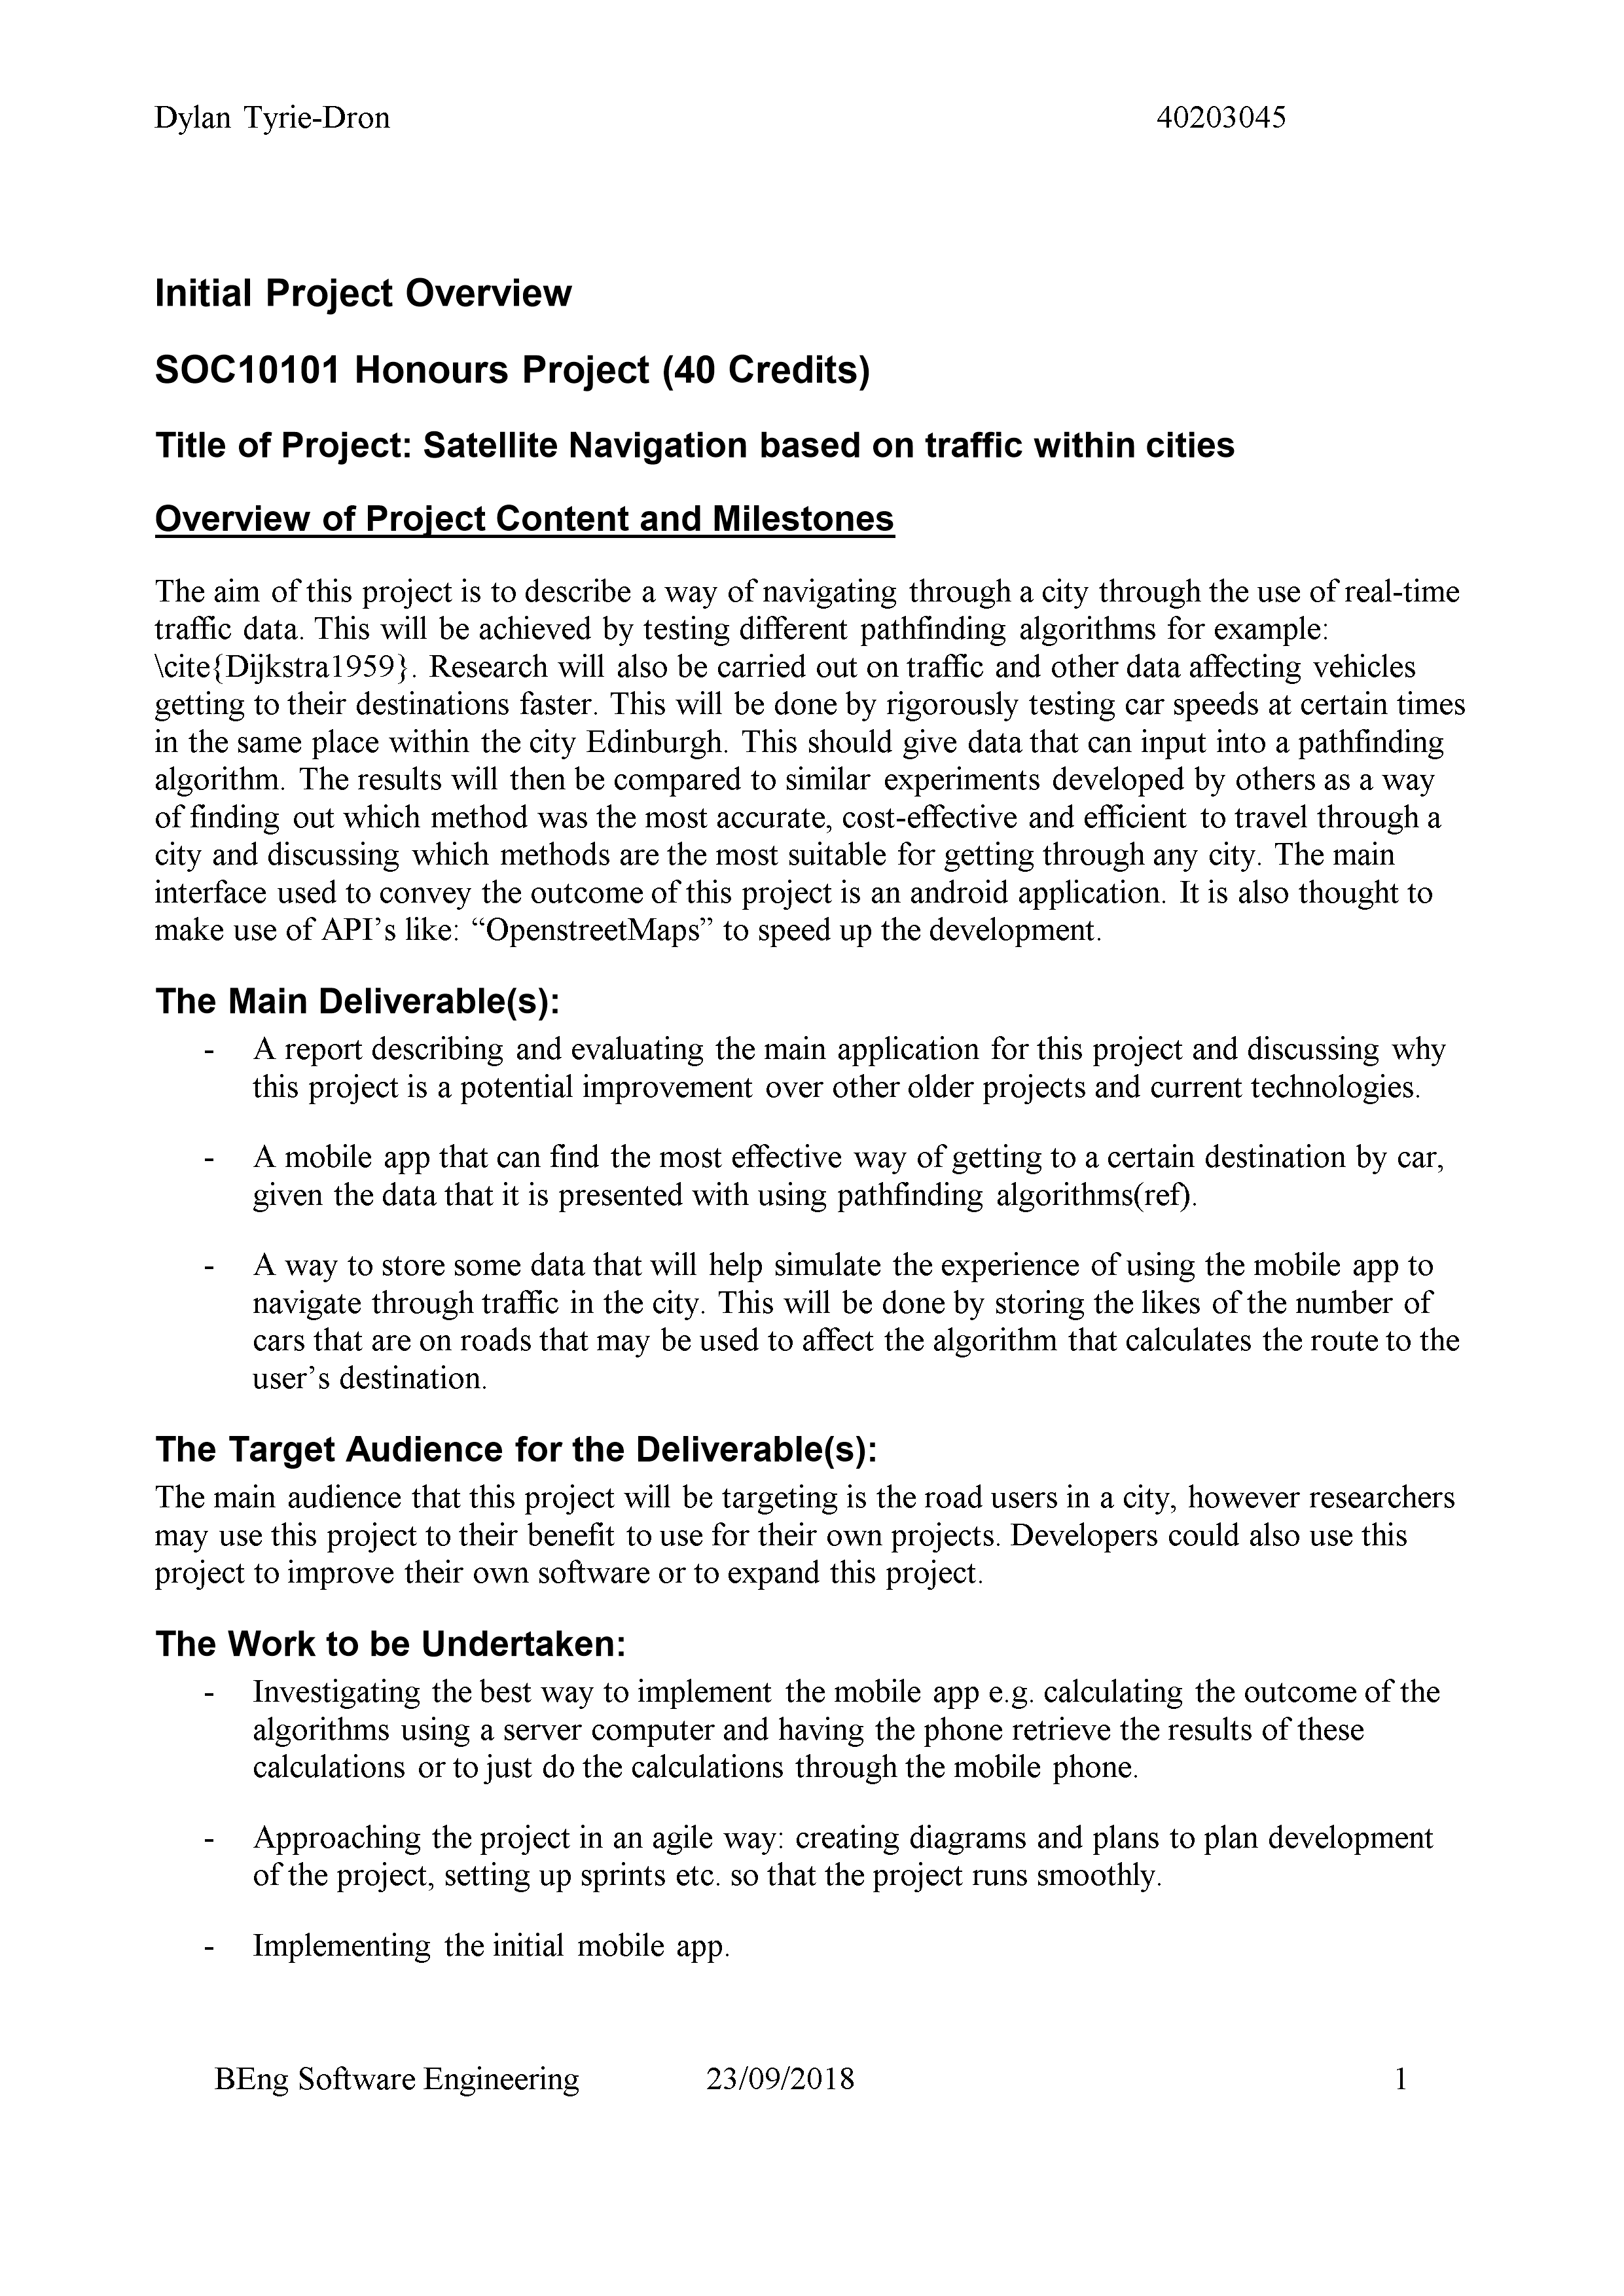
\includegraphics[width=\textwidth,height=\textheight,keepaspectratio]{IPOPage1.png} % fit images to page
\newpage
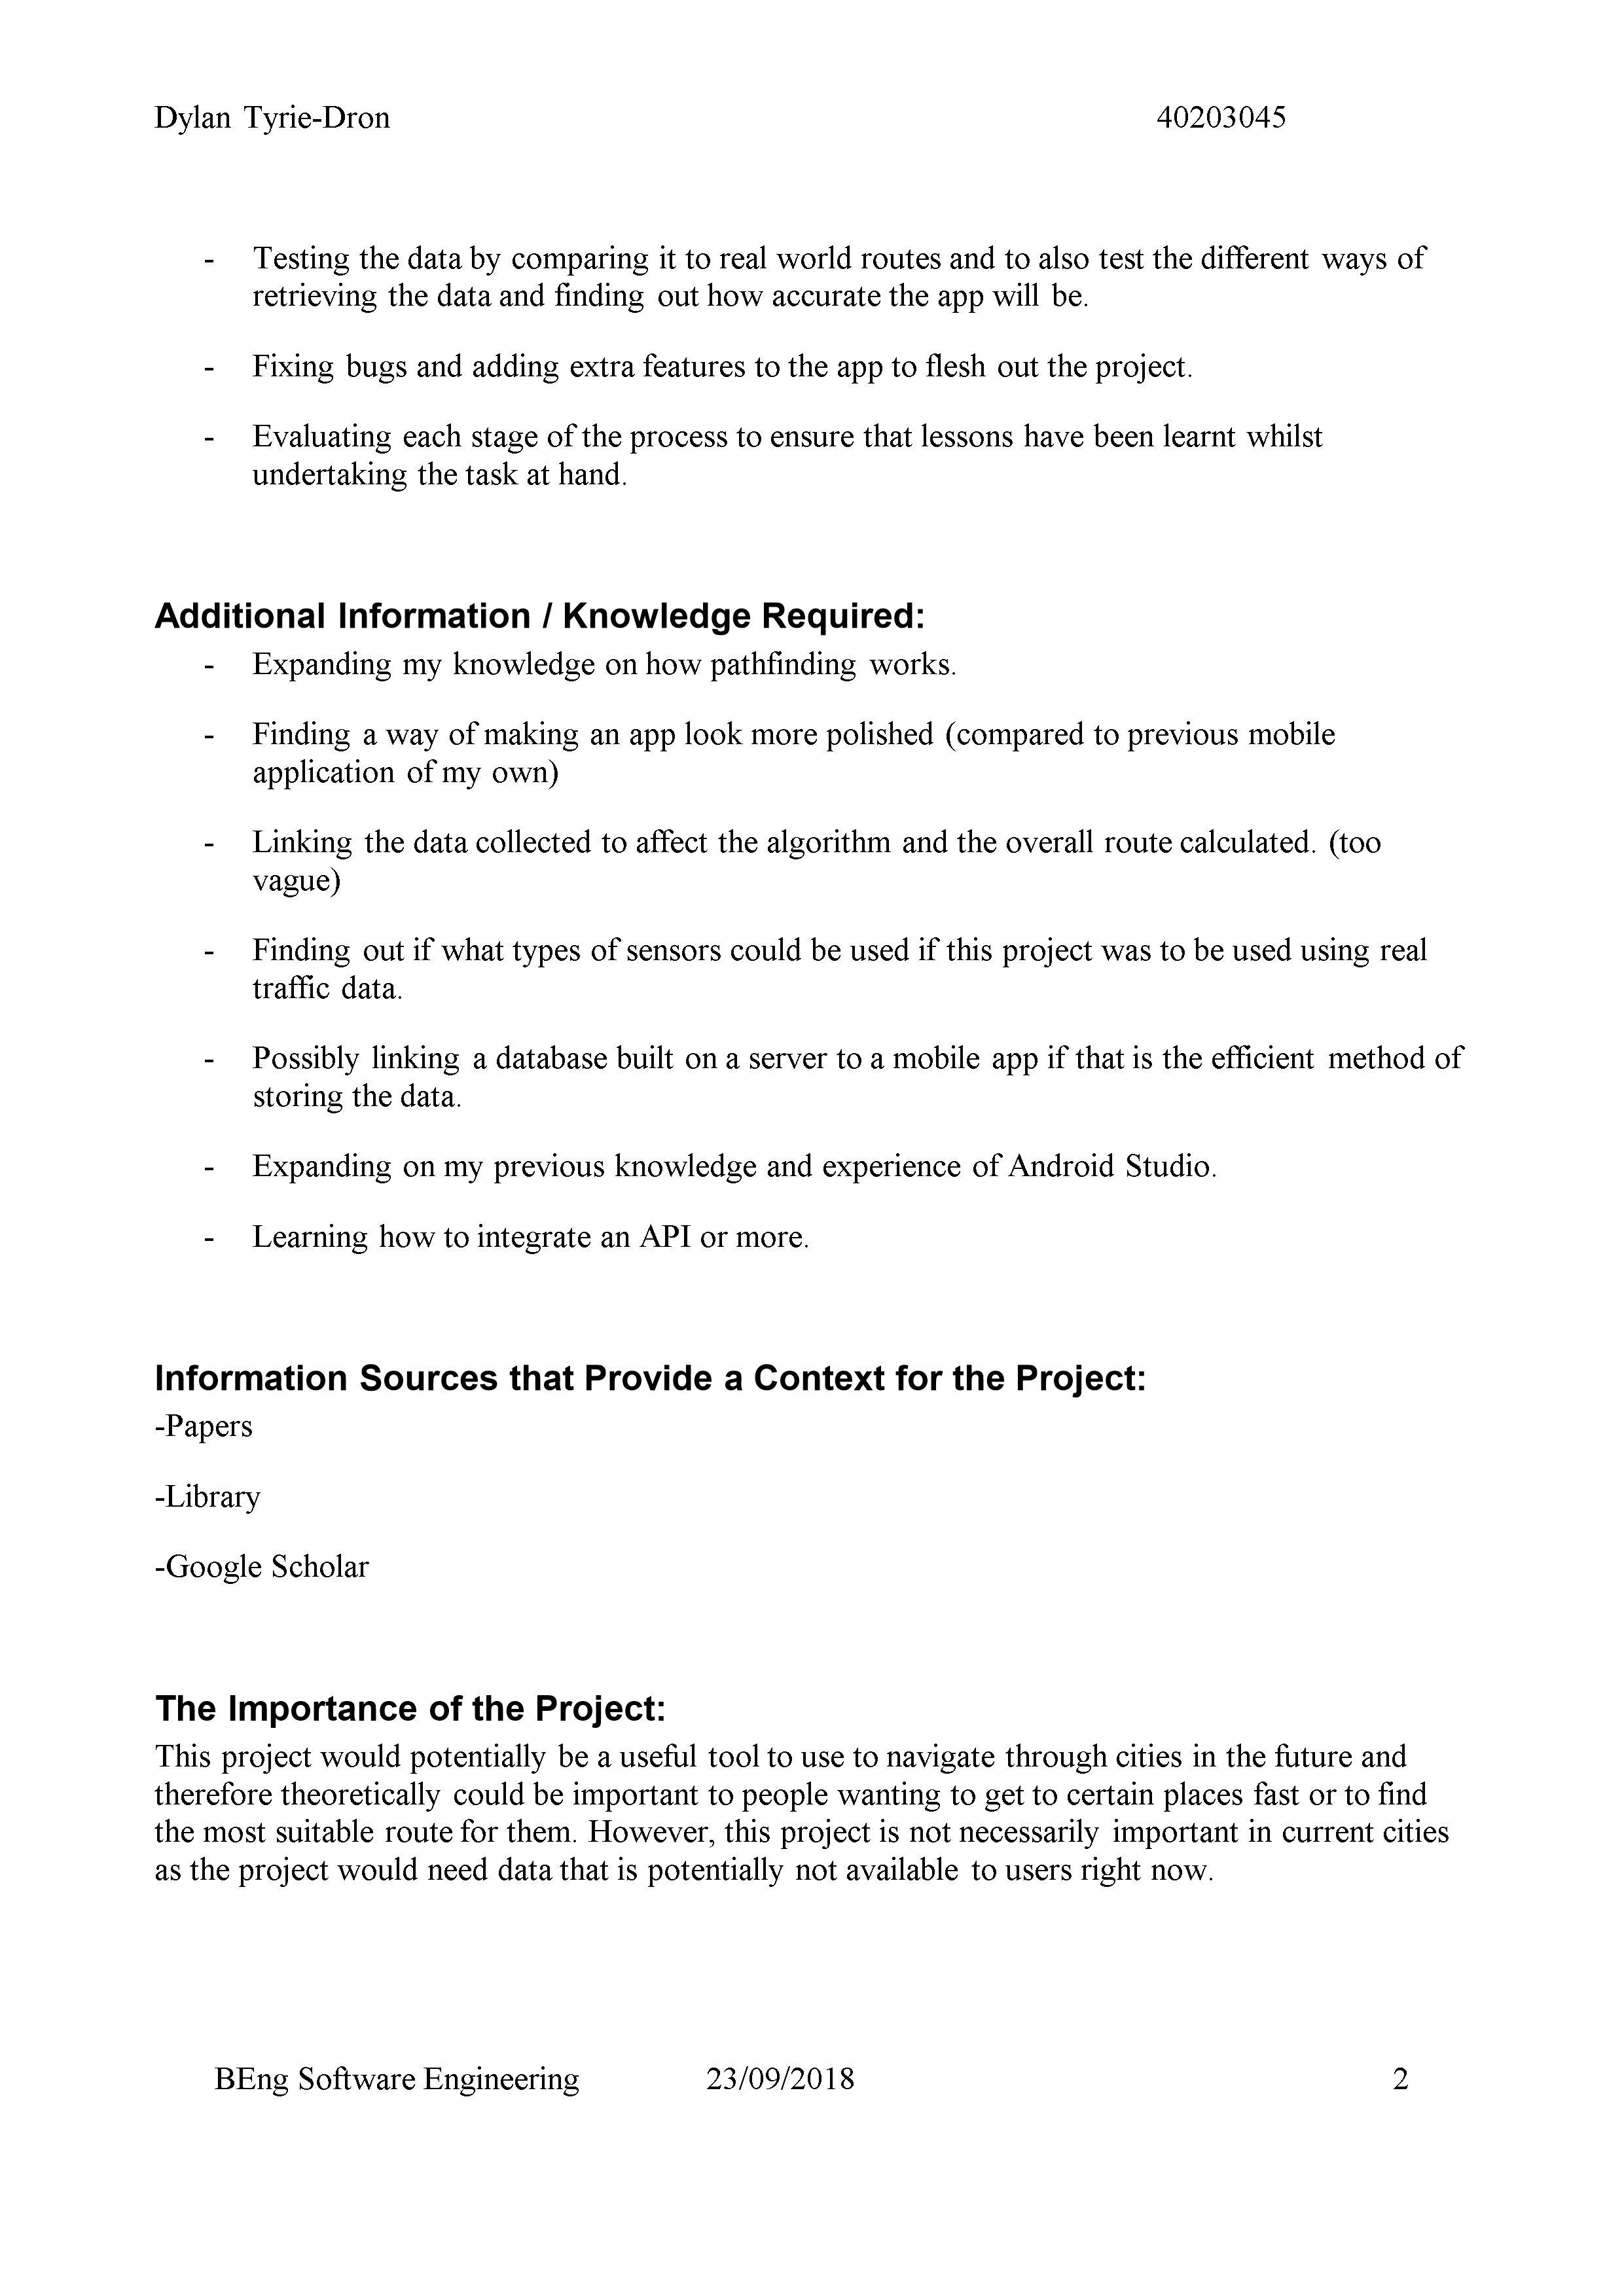
\includegraphics[width=\textwidth,height=\textheight,keepaspectratio]{IPOPage2.png}
\newpage

\includegraphics[width=\textwidth,height=\textheight,keepaspectratio]{IPOPage3.png} 
%insert IPO

% \begin{subappendices}
% \subsection{Example sub appendices}
% ...
% \end{subappendices}

% \section{Second Formal Review Output}
% Insert a copy of the project review form you were given at the end of the review by the second marker

 \section{Diary Sheets (or other project management evidence)}
% Insert diary sheets here together with any project management plan you have
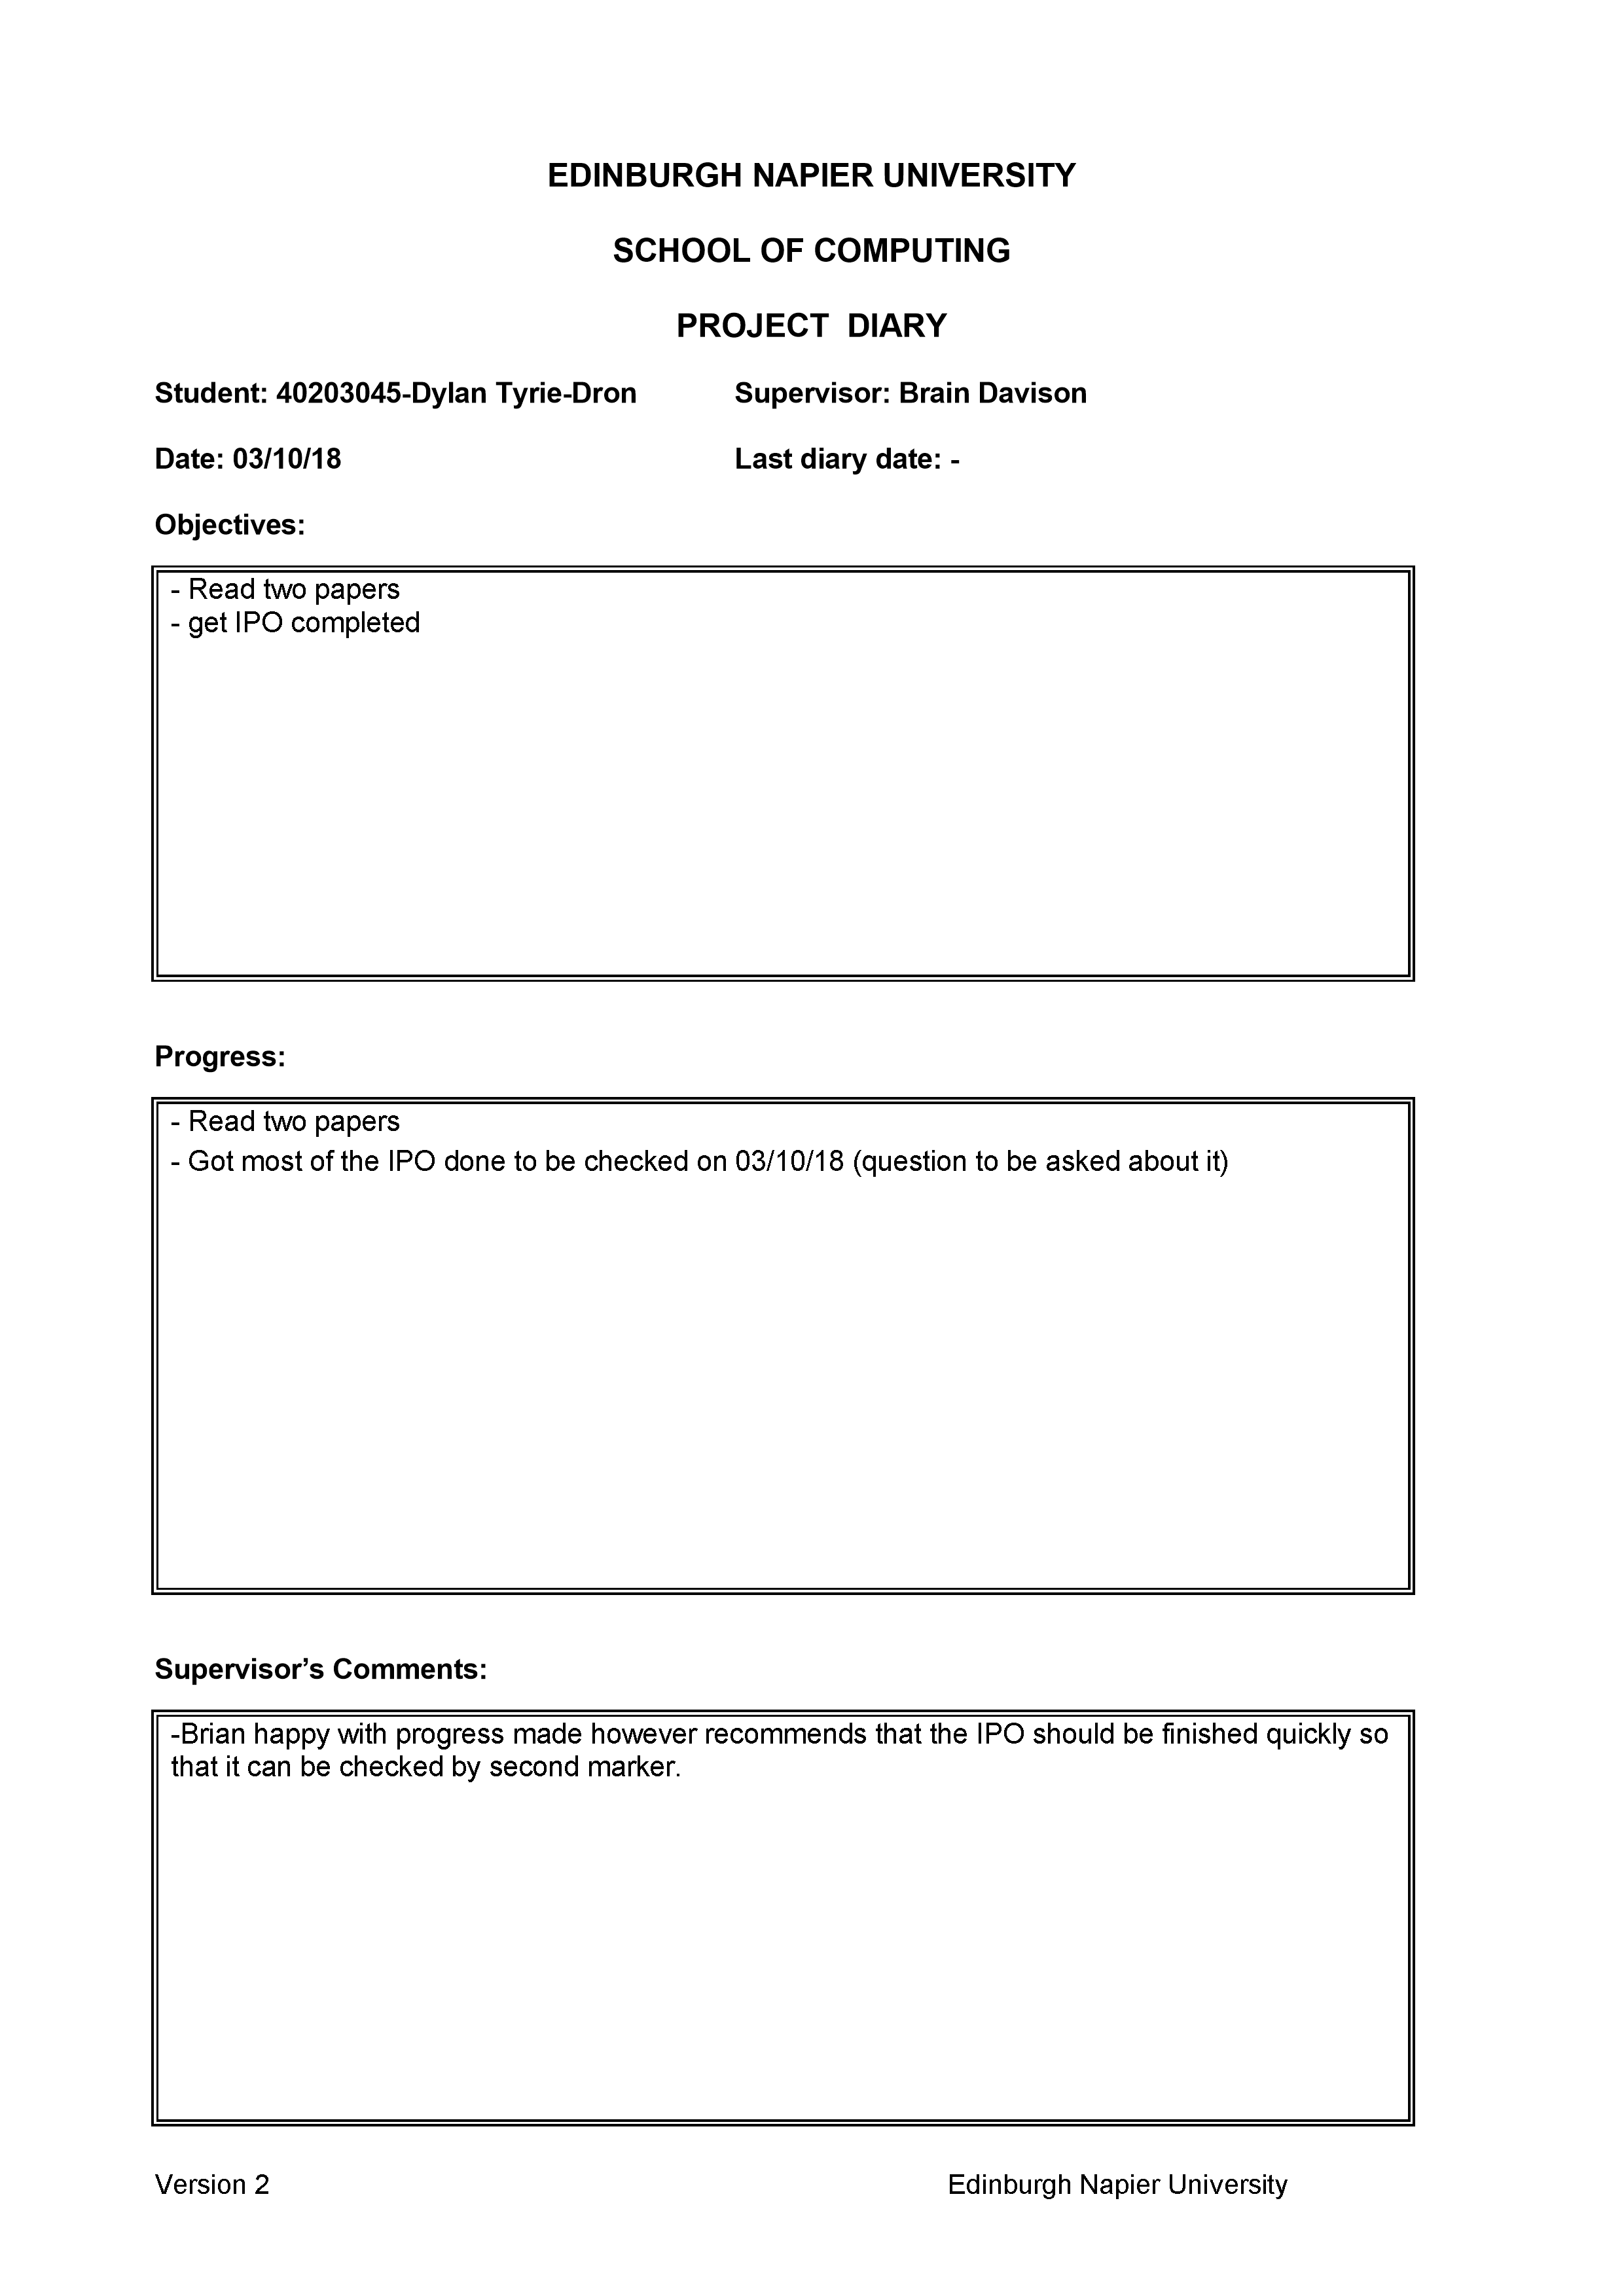
\includegraphics[width=\textwidth,height=\textheight,keepaspectratio]{diary1.png} % fit images to page
\newpage
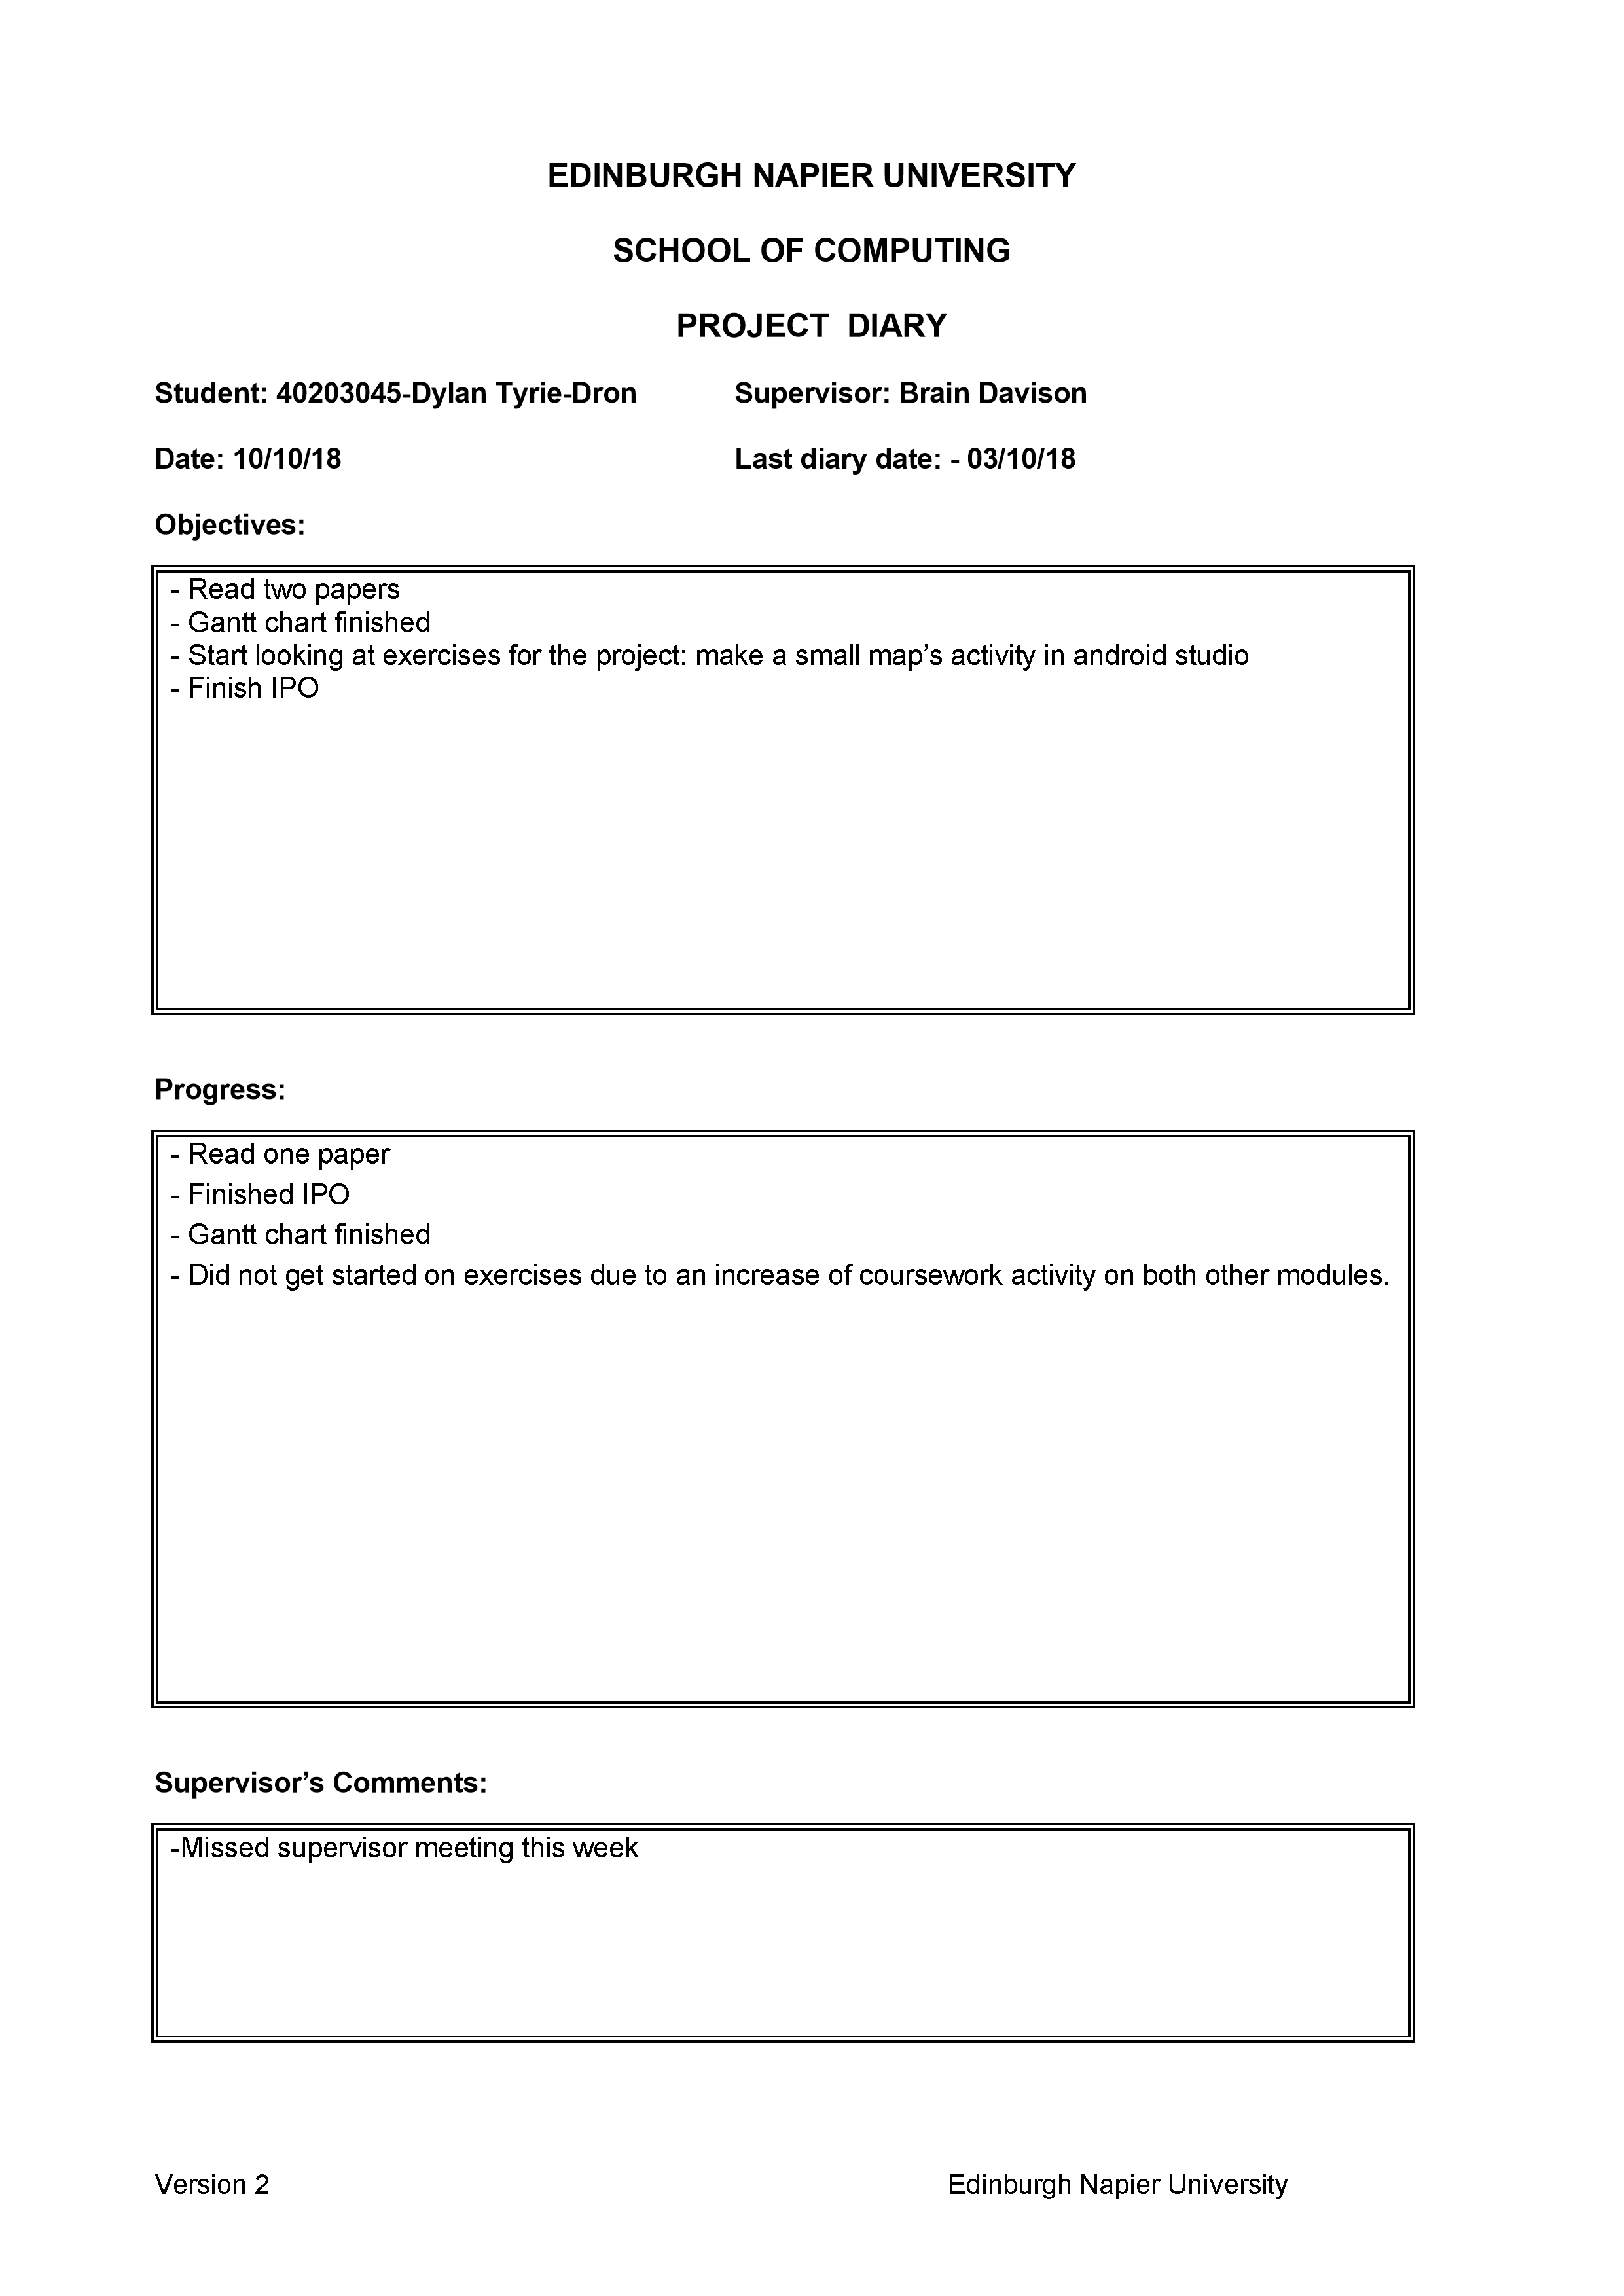
\includegraphics[width=\textwidth,height=\textheight,keepaspectratio]{diary2.png}
\newpage
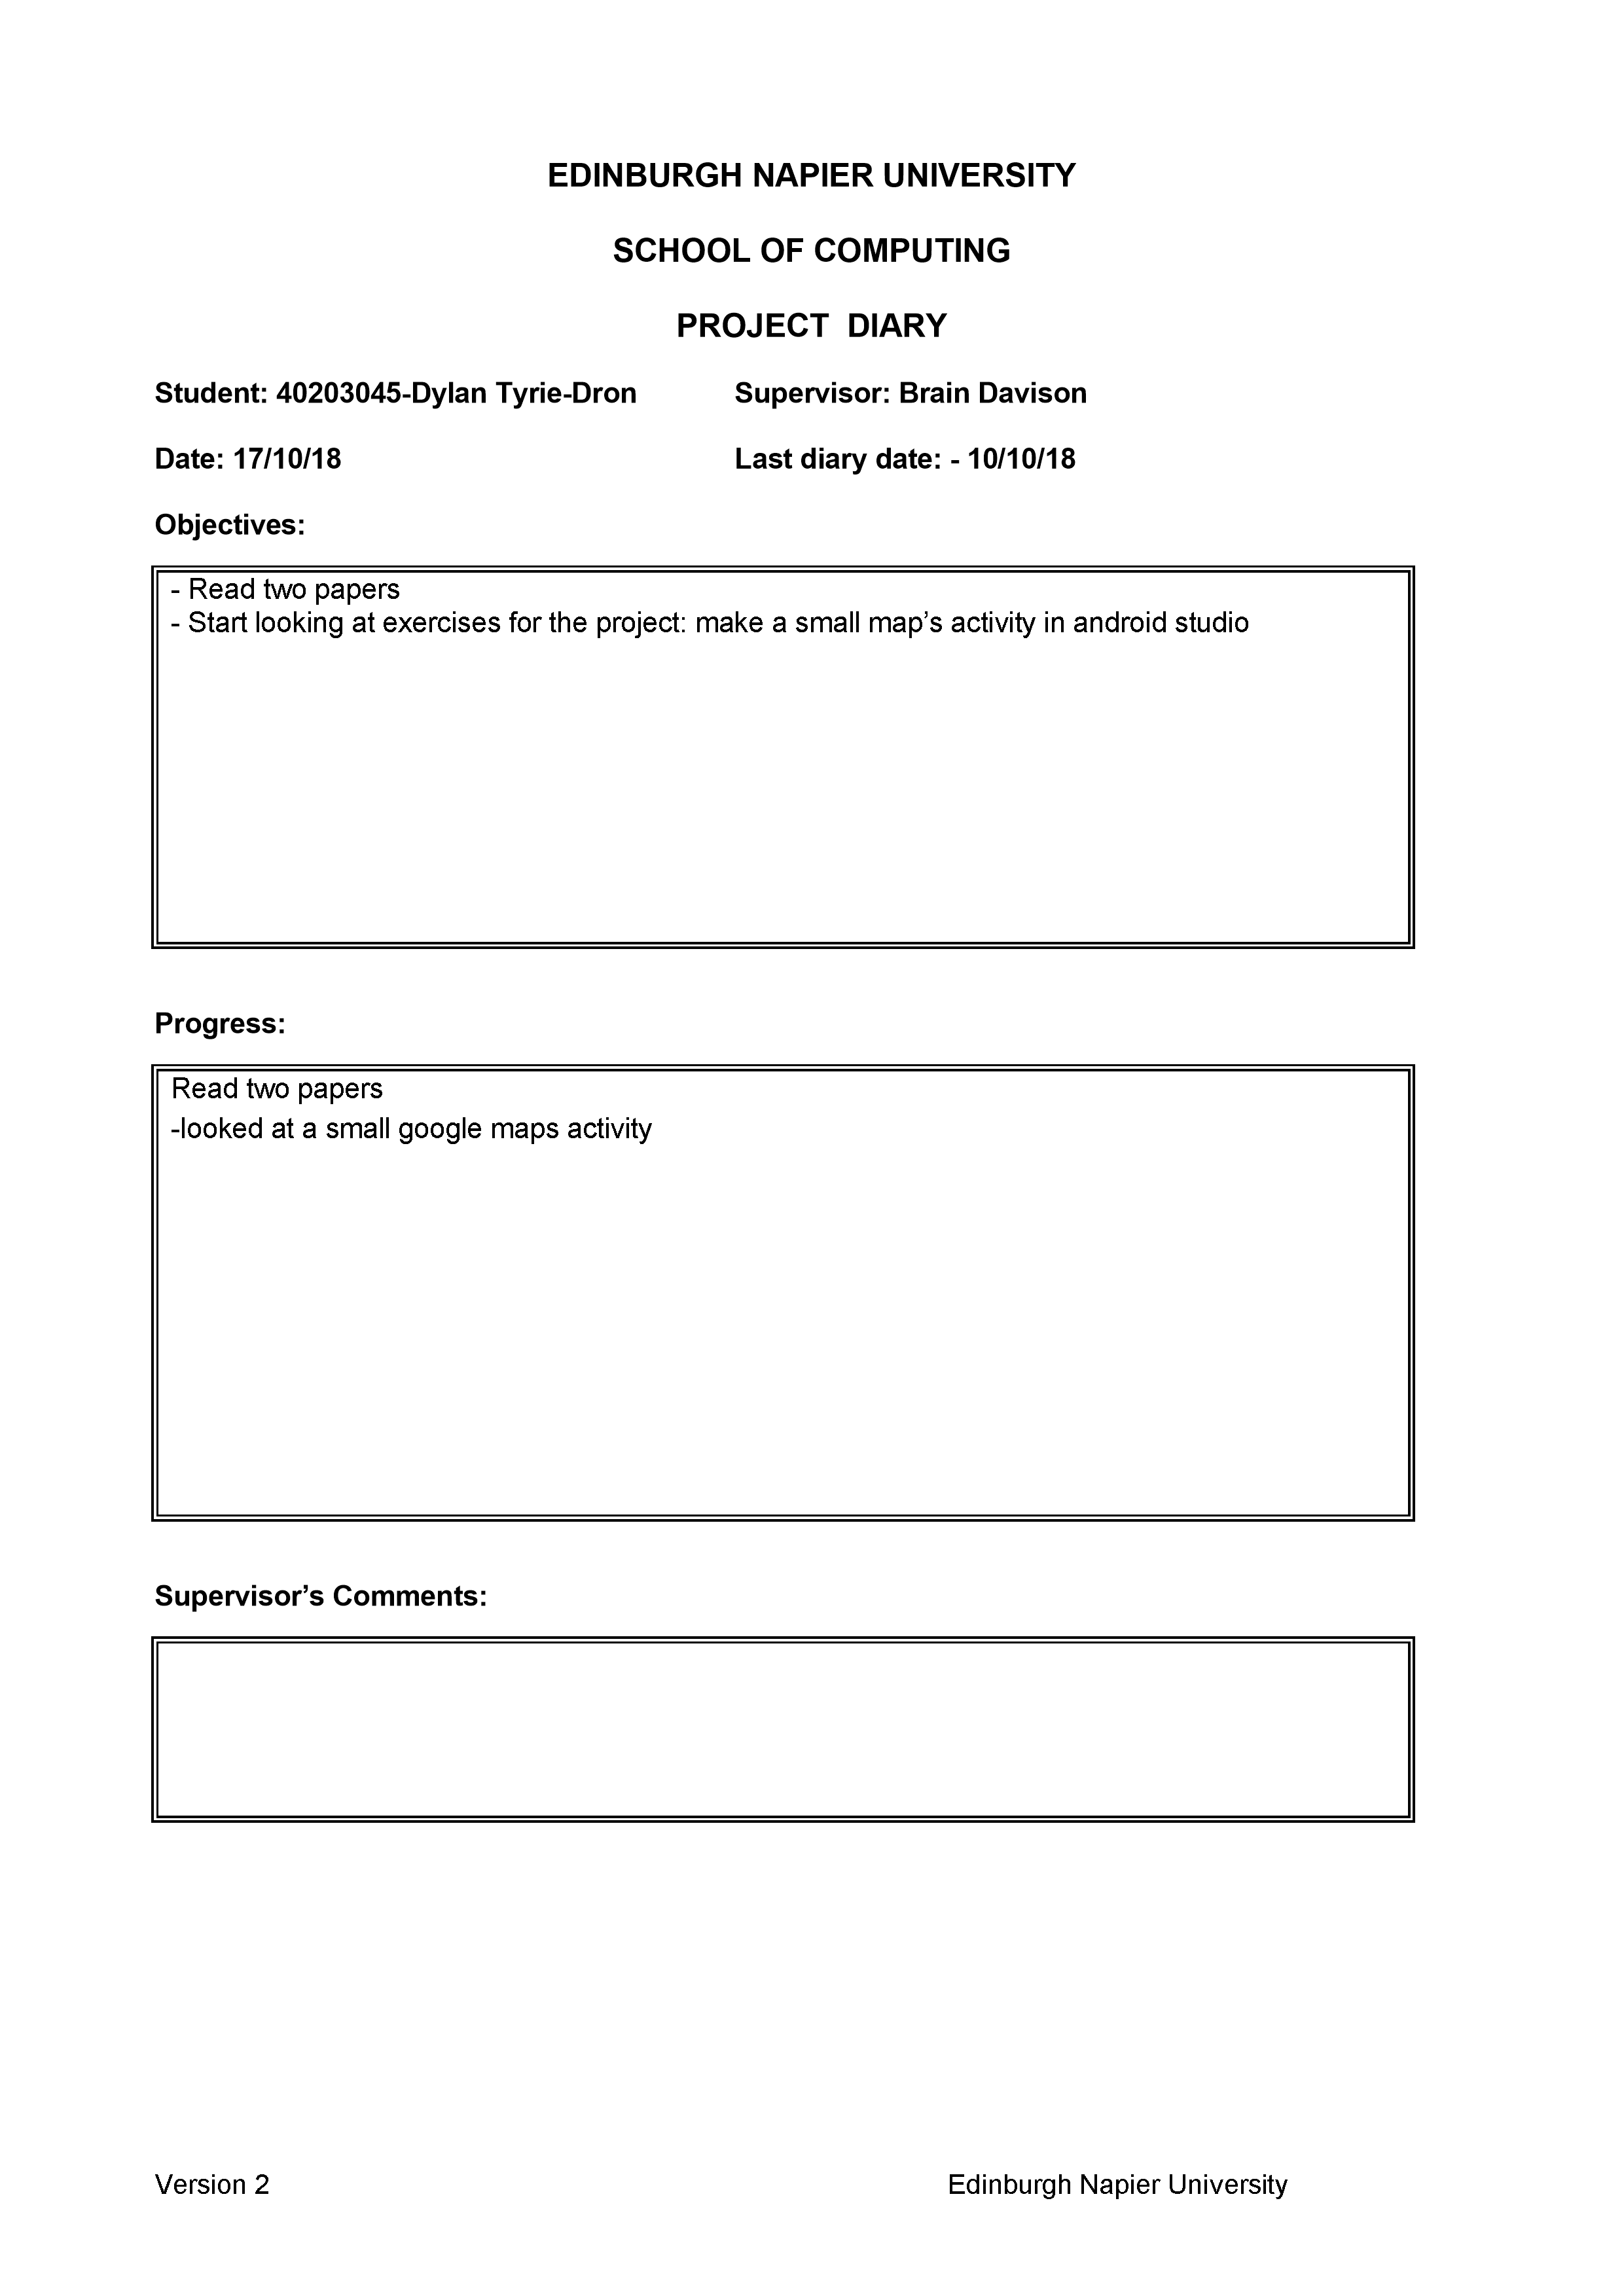
\includegraphics[width=\textwidth,height=\textheight,keepaspectratio]{diary3.png} 
\newpage
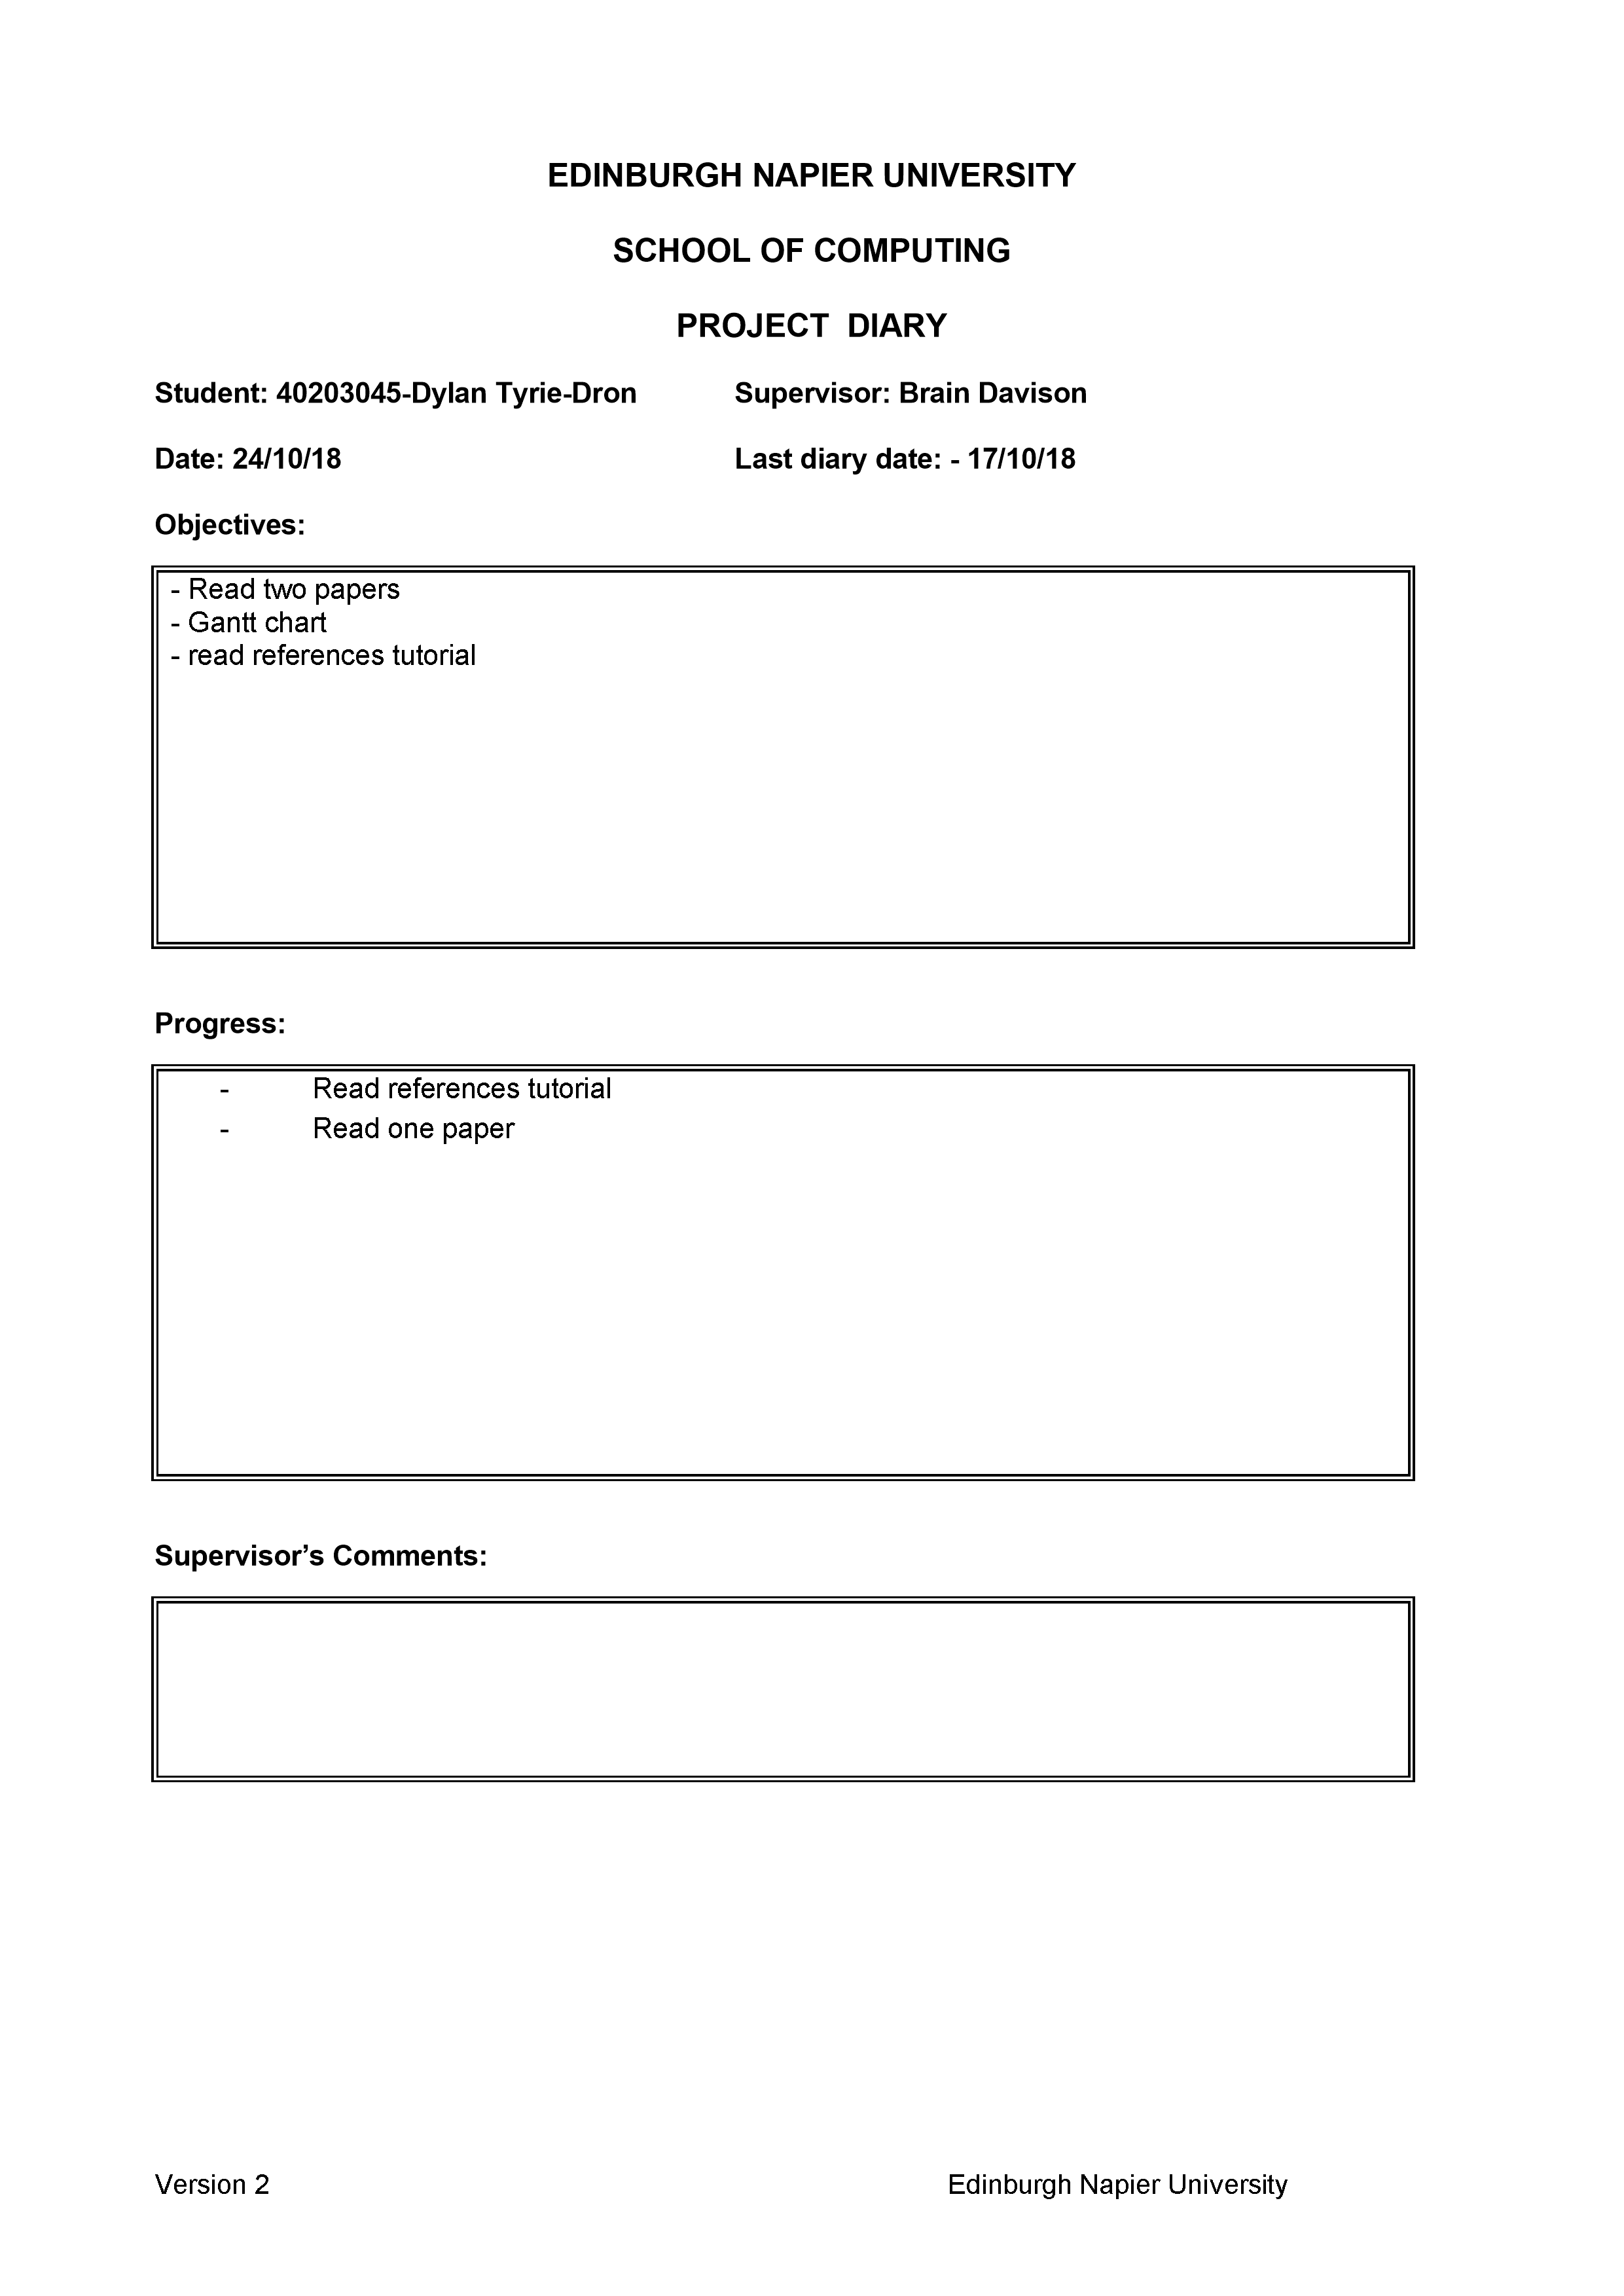
\includegraphics[width=\textwidth,height=\textheight,keepaspectratio]{diary4.png} 
\newpage
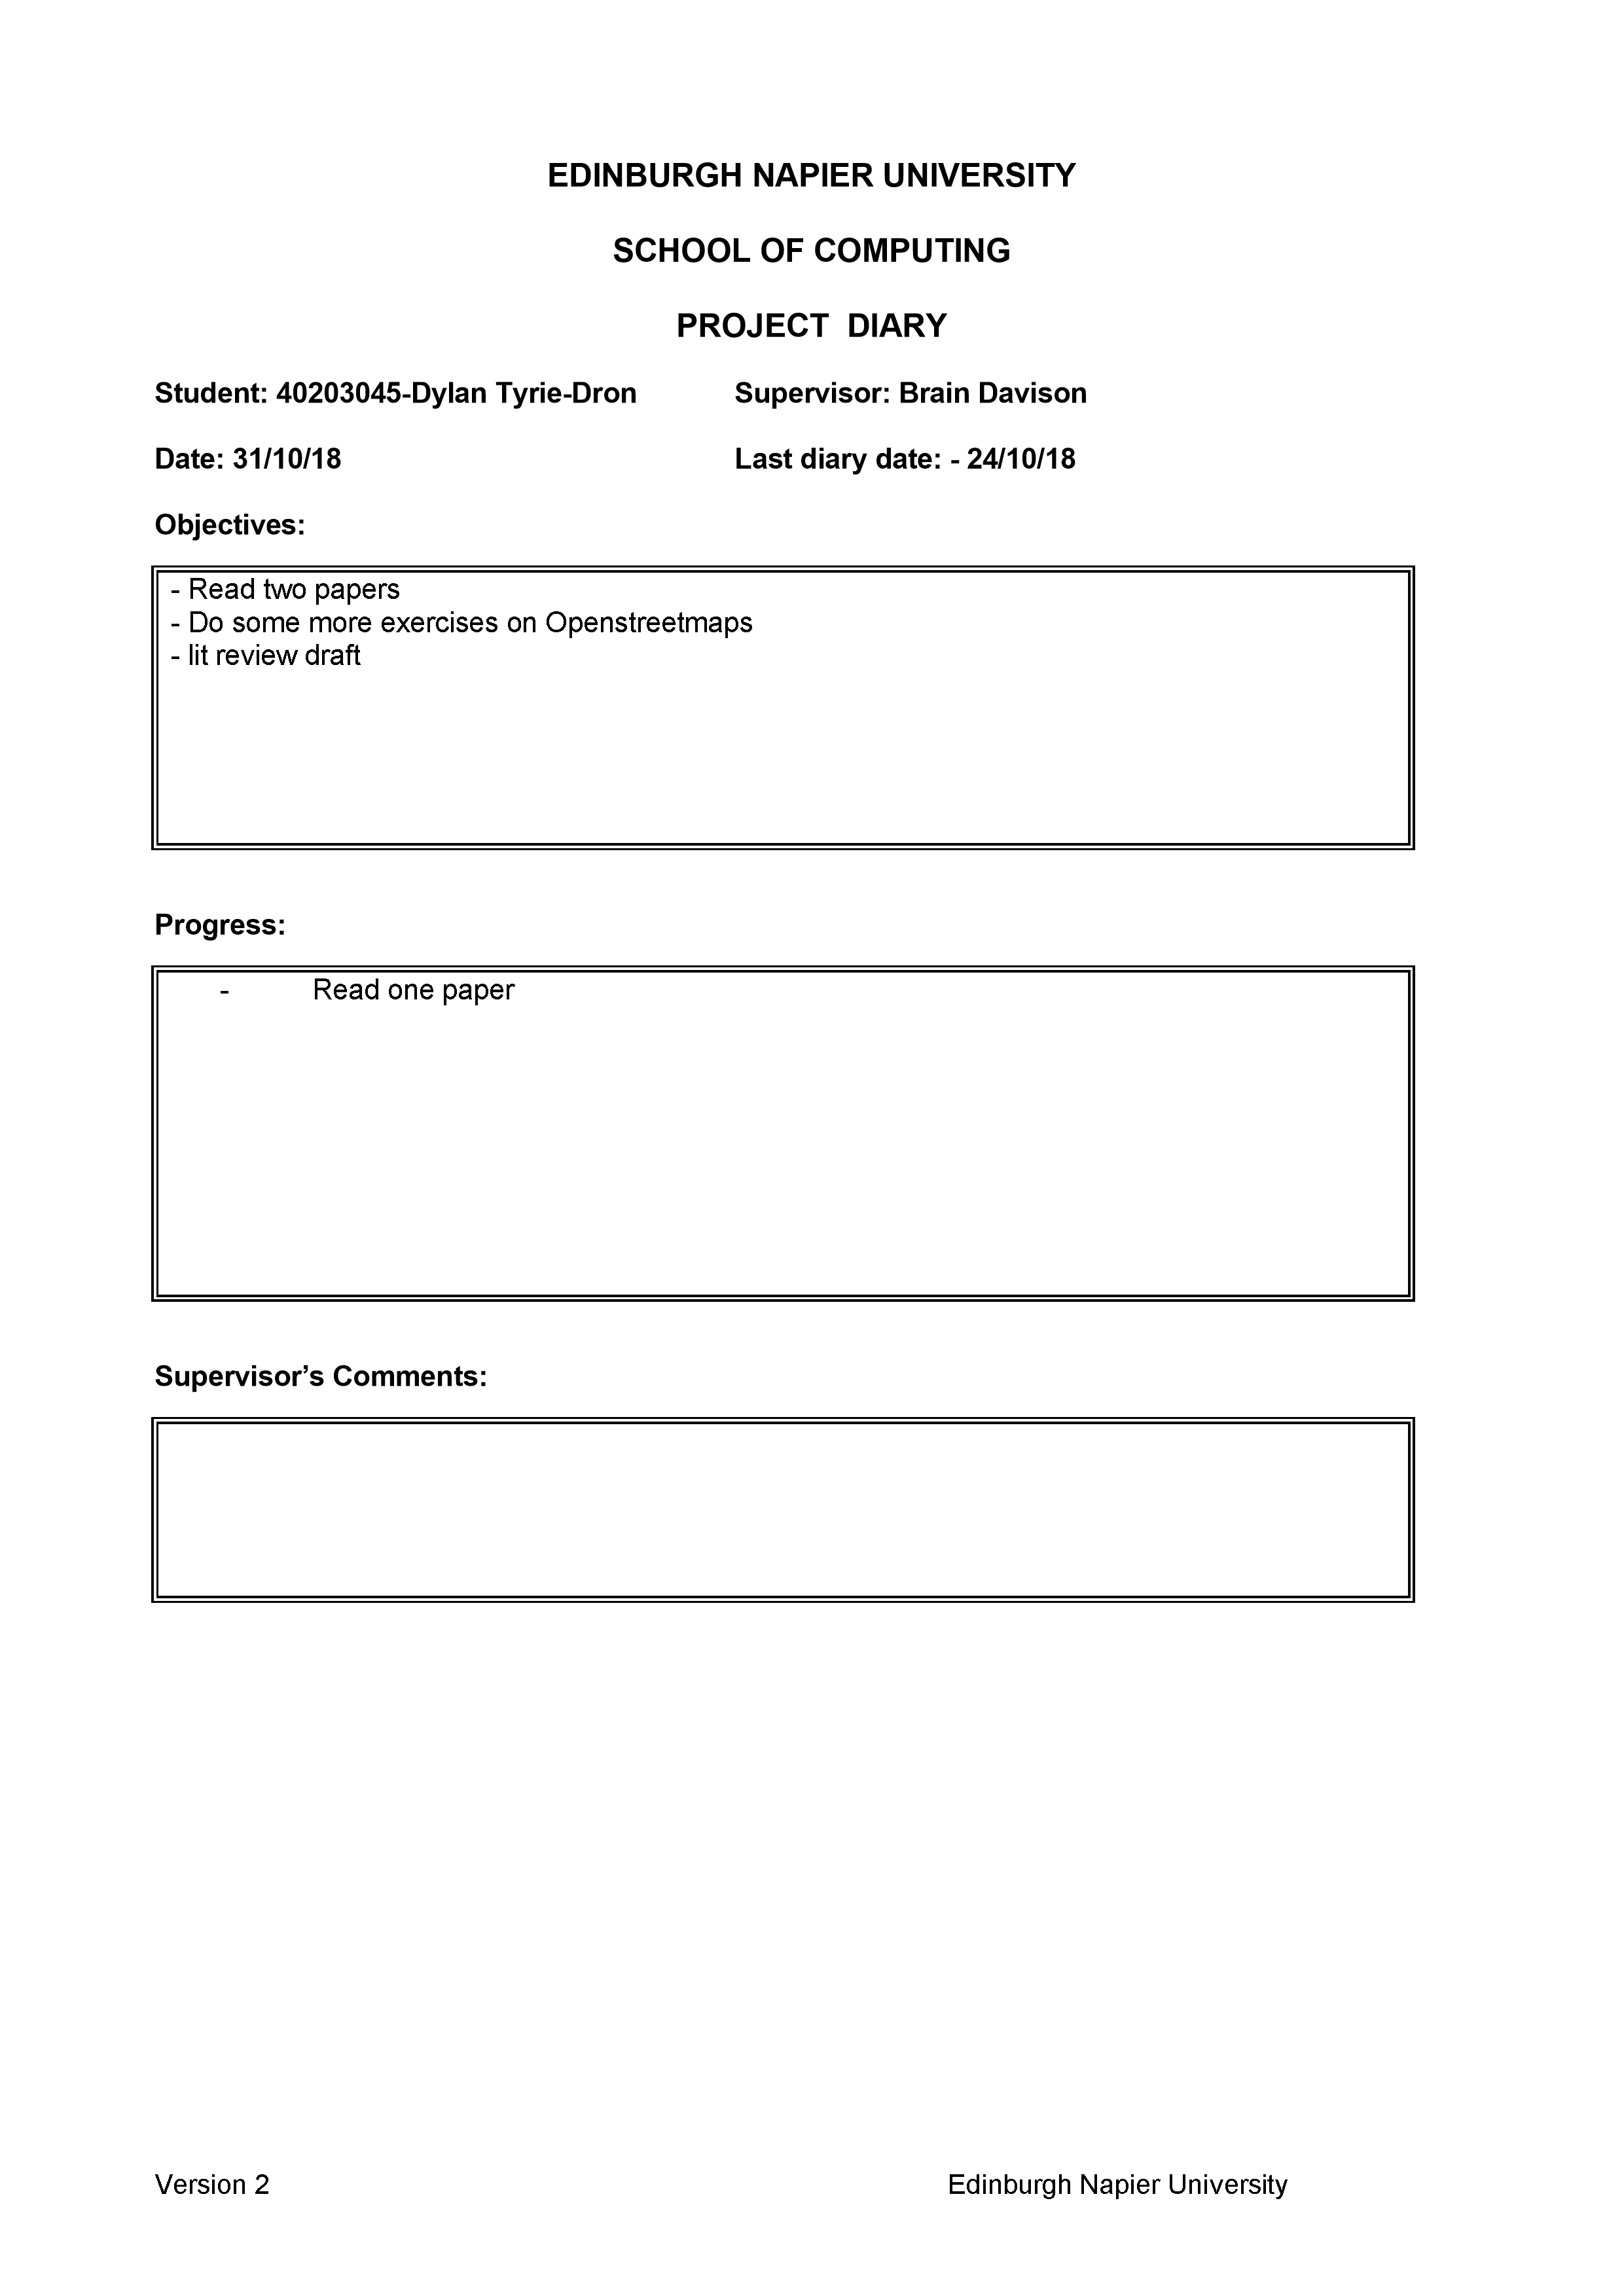
\includegraphics[width=\textwidth,height=\textheight,keepaspectratio]{diary5.png}
% \section{Appendix 4 and following}
% insert content here and for each of the other appendices, the title may be just on a page by itself, the pages of the appendices are not numbered, unless an included document such as a user manual or design document is itself pager numbered.
 \end{appendices}

\end{document}
